% Created 2024-01-15 Mon 16:55
% Intended LaTeX compiler: pdflatex
\documentclass[11pt]{article}
\usepackage[utf8]{inputenc}
\usepackage[T1]{fontenc}
\usepackage{graphicx}
\usepackage{longtable}
\usepackage{wrapfig}
\usepackage{rotating}
\usepackage[normalem]{ulem}
\usepackage{amsmath}
\usepackage{amssymb}
\usepackage{capt-of}
\usepackage{hyperref}
\graphicspath{{../../books/}}
% wrong resolution of image
% https://tex.stackexchange.com/questions/21627/image-from-includegraphics-showing-in-wrong-image-size?rq=1

%%%%%%%%%%%%%%%%%%%%%%%%%%%%%%%%%%%%%%
%% TIPS                                 %%
%%%%%%%%%%%%%%%%%%%%%%%%%%%%%%%%%%%%%%
% \substack{a\\b} for multiple lines text
% \usepackage{expl3}
% \expandafter\def\csname ver@l3regex.sty\endcsname{}
% \usepackage{pkgloader}
\usepackage[utf8]{inputenc}

% nfss error
% \usepackage[B1,T1]{fontenc}
\usepackage{fontspec}

% \usepackage[Emoticons]{ucharclasses}
\newfontfamily\DejaSans{DejaVu Sans}
% \setDefaultTransitions{\DejaSans}{}

% pdfplots will load xolor automatically without option
\usepackage[dvipsnames]{xcolor}

%                                                             ┳┳┓   ┓
%                                                             ┃┃┃┏┓╋┣┓
%                                                             ┛ ┗┗┻┗┛┗
% \usepackage{amsmath} mathtools loads the amsmath
\usepackage{amsmath}
\usepackage{mathtools}

\usepackage{amsthm}
\usepackage{amsbsy}

%\usepackage{commath}

\usepackage{amssymb}

\usepackage{mathrsfs}
%\usepackage{mathabx}
\usepackage{stmaryrd}
\usepackage{empheq}

\usepackage{scalerel}
\usepackage{stackengine}
\usepackage{stackrel}



\usepackage{nicematrix}
\usepackage{tensor}
\usepackage{blkarray}
\usepackage{siunitx}
\usepackage[f]{esvect}

% centering \not on a letter
\usepackage{slashed}
\usepackage[makeroom]{cancel}

%\usepackage{merriweather}
\usepackage{unicode-math}
\setmainfont{TeX Gyre Pagella}
% \setmathfont{STIX}
%\setmathfont{texgyrepagella-math.otf}
%\setmathfont{Libertinus Math}
\setmathfont{Latin Modern Math}

 % \setmathfont[range={\smwhtdiamond,\enclosediamond,\varlrtriangle}]{Latin Modern Math}
\setmathfont[range={\rightrightarrows,\twoheadrightarrow,\leftrightsquigarrow,\triangledown,\vartriangle,\precneq,\succneq,\prec,\succ,\preceq,\succeq,\tieconcat}]{XITS Math}
 \setmathfont[range={\int,\setminus}]{Libertinus Math}
 % \setmathfont[range={\mathalpha}]{TeX Gyre Pagella Math}
%\setmathfont[range={\mitA,\mitB,\mitC,\mitD,\mitE,\mitF,\mitG,\mitH,\mitI,\mitJ,\mitK,\mitL,\mitM,\mitN,\mitO,\mitP,\mitQ,\mitR,\mitS,\mitT,\mitU,\mitV,\mitW,\mitX,\mitY,\mitZ,\mita,\mitb,\mitc,\mitd,\mite,\mitf,\mitg,\miti,\mitj,\mitk,\mitl,\mitm,\mitn,\mito,\mitp,\mitq,\mitr,\mits,\mitt,\mitu,\mitv,\mitw,\mitx,\mity,\mitz}]{TeX Gyre Pagella Math}
% unicode is not good at this!
%\let\nmodels\nvDash

 \usepackage{wasysym}

 % for wide hat
 \DeclareSymbolFont{yhlargesymbols}{OMX}{yhex}{m}{n} \DeclareMathAccent{\what}{\mathord}{yhlargesymbols}{"62}

%                                                               ┏┳┓•┓
%                                                                ┃ ┓┃┏┓
%                                                                ┻ ┗┛┗┗

\usepackage{pgfplots}
\pgfplotsset{compat=1.18}
\usepackage{tikz}
\usepackage{tikz-cd}
\tikzcdset{scale cd/.style={every label/.append style={scale=#1},
    cells={nodes={scale=#1}}}}
% TODO: discard qtree and use forest
% \usepackage{tikz-qtree}
\usepackage{forest}

\usetikzlibrary{arrows,positioning,calc,fadings,decorations,matrix,decorations,shapes.misc}
%setting from geogebra
\definecolor{ccqqqq}{rgb}{0.8,0,0}

%                                                          ┳┳┓•    ┓┓
%                                                          ┃┃┃┓┏┏┏┓┃┃┏┓┏┓┏┓┏┓┓┏┏
%                                                          ┛ ┗┗┛┗┗ ┗┗┗┻┛┗┗ ┗┛┗┻┛
%\usepackage{twemojis}
\usepackage[most]{tcolorbox}
\usepackage{threeparttable}
\usepackage{tabularx}

\usepackage{enumitem}
\usepackage[indLines=false]{algpseudocodex}
\usepackage[]{algorithm2e}
% \SetKwComment{Comment}{/* }{ */}
% \algrenewcommand\algorithmicrequire{\textbf{Input:}}
% \algrenewcommand\algorithmicensure{\textbf{Output:}}
% wrong with preview
\usepackage{subcaption}
\usepackage{caption}
% {\aunclfamily\Huge}
\usepackage{auncial}

\usepackage{float}

\usepackage{fancyhdr}

\usepackage{ifthen}
\usepackage{xargs}

\definecolor{mintedbg}{rgb}{0.99,0.99,0.99}
\usepackage[cachedir=\detokenize{~/miscellaneous/trash}]{minted}
\setminted{breaklines,
  mathescape,
  bgcolor=mintedbg,
  fontsize=\footnotesize,
  frame=single,
  linenos}
\usemintedstyle{xcode}
\usepackage{tcolorbox}
\usepackage{etoolbox}



\usepackage{imakeidx}
\usepackage{hyperref}
\usepackage{soul}
\usepackage{framed}

% don't use this for preview
%\usepackage[margin=1.5in]{geometry}
% \usepackage{geometry}
% \geometry{legalpaper, landscape, margin=1in}
\usepackage[font=itshape]{quoting}

%\LoadPackagesNow
%\usepackage[xetex]{preview}
%%%%%%%%%%%%%%%%%%%%%%%%%%%%%%%%%%%%%%%
%% USEPACKAGES end                       %%
%%%%%%%%%%%%%%%%%%%%%%%%%%%%%%%%%%%%%%%

%%%%%%%%%%%%%%%%%%%%%%%%%%%%%%%%%%%%%%%
%% Algorithm environment
%%%%%%%%%%%%%%%%%%%%%%%%%%%%%%%%%%%%%%%
\SetKwIF{Recv}{}{}{upon receiving}{do}{}{}{}
\SetKwBlock{Init}{initially do}{}
\SetKwProg{Function}{Function}{:}{}

% https://github.com/chrmatt/algpseudocodex/issues/3
\algnewcommand\algorithmicswitch{\textbf{switch}}%
\algnewcommand\algorithmiccase{\textbf{case}}
\algnewcommand\algorithmicof{\textbf{of}}
\algnewcommand\algorithmicotherwise{\texttt{otherwise} $\Rightarrow$}

\makeatletter
\algdef{SE}[SWITCH]{Switch}{EndSwitch}[1]{\algpx@startIndent\algpx@startCodeCommand\algorithmicswitch\ #1\ \algorithmicdo}{\algpx@endIndent\algpx@startCodeCommand\algorithmicend\ \algorithmicswitch}%
\algdef{SE}[CASE]{Case}{EndCase}[1]{\algpx@startIndent\algpx@startCodeCommand\algorithmiccase\ #1}{\algpx@endIndent\algpx@startCodeCommand\algorithmicend\ \algorithmiccase}%
\algdef{SE}[CASEOF]{CaseOf}{EndCaseOf}[1]{\algpx@startIndent\algpx@startCodeCommand\algorithmiccase\ #1 \algorithmicof}{\algpx@endIndent\algpx@startCodeCommand\algorithmicend\ \algorithmiccase}
\algdef{SE}[OTHERWISE]{Otherwise}{EndOtherwise}[0]{\algpx@startIndent\algpx@startCodeCommand\algorithmicotherwise}{\algpx@endIndent\algpx@startCodeCommand\algorithmicend\ \algorithmicotherwise}
\ifbool{algpx@noEnd}{%
  \algtext*{EndSwitch}%
  \algtext*{EndCase}%
  \algtext*{EndCaseOf}
  \algtext*{EndOtherwise}
  %
  % end indent line after (not before), to get correct y position for multiline text in last command
  \apptocmd{\EndSwitch}{\algpx@endIndent}{}{}%
  \apptocmd{\EndCase}{\algpx@endIndent}{}{}%
  \apptocmd{\EndCaseOf}{\algpx@endIndent}{}{}
  \apptocmd{\EndOtherwise}{\algpx@endIndent}{}{}
}{}%

\pretocmd{\Switch}{\algpx@endCodeCommand}{}{}
\pretocmd{\Case}{\algpx@endCodeCommand}{}{}
\pretocmd{\CaseOf}{\algpx@endCodeCommand}{}{}
\pretocmd{\Otherwise}{\algpx@endCodeCommand}{}{}

% for end commands that may not be printed, tell endCodeCommand whether we are using noEnd
\ifbool{algpx@noEnd}{%
  \pretocmd{\EndSwitch}{\algpx@endCodeCommand[1]}{}{}%
  \pretocmd{\EndCase}{\algpx@endCodeCommand[1]}{}{}
  \pretocmd{\EndCaseOf}{\algpx@endCodeCommand[1]}{}{}%
  \pretocmd{\EndOtherwise}{\algpx@endCodeCommand[1]}{}{}
}{%
  \pretocmd{\EndSwitch}{\algpx@endCodeCommand[0]}{}{}%
  \pretocmd{\EndCase}{\algpx@endCodeCommand[0]}{}{}%
  \pretocmd{\EndCaseOf}{\algpx@endCodeCommand[0]}{}{}
  \pretocmd{\EndOtherwise}{\algpx@endCodeCommand[0]}{}{}
}%
\makeatother
% % For algpseudocode
% \algnewcommand\algorithmicswitch{\textbf{switch}}
% \algnewcommand\algorithmiccase{\textbf{case}}
% \algnewcommand\algorithmiccaseof{\textbf{case}}
% \algnewcommand\algorithmicof{\textbf{of}}
% % New "environments"
% \algdef{SE}[SWITCH]{Switch}{EndSwitch}[1]{\algorithmicswitch\ #1\ \algorithmicdo}{\algorithmicend\ \algorithmicswitch}%
% \algdef{SE}[CASE]{Case}{EndCase}[1]{\algorithmiccase\ #1}{\algorithmicend\ \algorithmiccase}%
% \algtext*{EndSwitch}%
% \algtext*{EndCase}
% \algdef{SE}[CASEOF]{CaseOf}{EndCaseOf}[1]{\algorithmiccaseof\ #1 \algorithmicof}{\algorithmicend\ \algorithmiccaseof}
% \algtext*{EndCaseOf}



%\pdfcompresslevel0

% quoting from
% https://tex.stackexchange.com/questions/391726/the-quotation-environment
\NewDocumentCommand{\bywhom}{m}{% the Bourbaki trick
  {\nobreak\hfill\penalty50\hskip1em\null\nobreak
   \hfill\mbox{\normalfont(#1)}%
   \parfillskip=0pt \finalhyphendemerits=0 \par}%
}

\NewDocumentEnvironment{pquotation}{m}
  {\begin{quoting}[
     indentfirst=true,
     leftmargin=\parindent,
     rightmargin=\parindent]\itshape}
  {\bywhom{#1}\end{quoting}}

\indexsetup{othercode=\small}
\makeindex[columns=2,options={-s /media/wu/file/stuuudy/notes/index_style.ist},intoc]
\makeatletter
\def\@idxitem{\par\hangindent 0pt}
\makeatother


% \newcounter{dummy} \numberwithin{dummy}{section}
\newtheorem{dummy}{dummy}[section]
\theoremstyle{definition}
\newtheorem{definition}[dummy]{Definition}
\theoremstyle{plain}
\newtheorem{corollary}[dummy]{Corollary}
\newtheorem{lemma}[dummy]{Lemma}
\newtheorem{proposition}[dummy]{Proposition}
\newtheorem{theorem}[dummy]{Theorem}
\newtheorem{notation}[dummy]{Notation}
\newtheorem{conjecture}[dummy]{Conjecture}
\newtheorem{fact}[dummy]{Fact}
\newtheorem{warning}[dummy]{Warning}
\theoremstyle{definition}
\newtheorem{examplle}{Example}[section]
\theoremstyle{remark}
\newtheorem*{remark}{Remark}
\newtheorem{exercise}{Exercise}[subsection]
\newtheorem{problem}{Problem}[subsection]
\newtheorem{observation}{Observation}[section]
\newenvironment{claim}[1]{\par\noindent\textbf{Claim:}\space#1}{}

\makeatletter
\DeclareFontFamily{U}{tipa}{}
\DeclareFontShape{U}{tipa}{m}{n}{<->tipa10}{}
\newcommand{\arc@char}{{\usefont{U}{tipa}{m}{n}\symbol{62}}}%

\newcommand{\arc}[1]{\mathpalette\arc@arc{#1}}

\newcommand{\arc@arc}[2]{%
  \sbox0{$\m@th#1#2$}%
  \vbox{
    \hbox{\resizebox{\wd0}{\height}{\arc@char}}
    \nointerlineskip
    \box0
  }%
}
\makeatother

\setcounter{MaxMatrixCols}{20}
%%%%%%% ABS
\DeclarePairedDelimiter\abss{\lvert}{\rvert}%
\DeclarePairedDelimiter\normm{\lVert}{\rVert}%

% Swap the definition of \abs* and \norm*, so that \abs
% and \norm resizes the size of the brackets, and the
% starred version does not.
\makeatletter
\let\oldabs\abss
%\def\abs{\@ifstar{\oldabs}{\oldabs*}}
\newcommand{\abs}{\@ifstar{\oldabs}{\oldabs*}}
\newcommand{\norm}[1]{\left\lVert#1\right\rVert}
%\let\oldnorm\normm
%\def\norm{\@ifstar{\oldnorm}{\oldnorm*}}
%\renewcommand{norm}{\@ifstar{\oldnorm}{\oldnorm*}}
\makeatother

% \stackMath
% \newcommand\what[1]{%
% \savestack{\tmpbox}{\stretchto{%
%   \scaleto{%
%     \scalerel*[\widthof{\ensuremath{#1}}]{\kern-.6pt\bigwedge\kern-.6pt}%
%     {\rule[-\textheight/2]{1ex}{\textheight}}%WIDTH-LIMITED BIG WEDGE
%   }{\textheight}%
% }{0.5ex}}%
% \stackon[1pt]{#1}{\tmpbox}%
% }

% \newcommand\what[1]{\ThisStyle{%
%     \setbox0=\hbox{$\SavedStyle#1$}%
%     \stackengine{-1.0\ht0+.5pt}{$\SavedStyle#1$}{%
%       \stretchto{\scaleto{\SavedStyle\mkern.15mu\char'136}{2.6\wd0}}{1.4\ht0}%
%     }{O}{c}{F}{T}{S}%
%   }
% }

% \newcommand\wtilde[1]{\ThisStyle{%
%     \setbox0=\hbox{$\SavedStyle#1$}%
%     \stackengine{-.1\LMpt}{$\SavedStyle#1$}{%
%       \stretchto{\scaleto{\SavedStyle\mkern.2mu\AC}{.5150\wd0}}{.6\ht0}%
%     }{O}{c}{F}{T}{S}%
%   }
% }

% \newcommand\wbar[1]{\ThisStyle{%
%     \setbox0=\hbox{$\SavedStyle#1$}%
%     \stackengine{.5pt+\LMpt}{$\SavedStyle#1$}{%
%       \rule{\wd0}{\dimexpr.3\LMpt+.3pt}%
%     }{O}{c}{F}{T}{S}%
%   }
% }

\newcommand{\bl}[1] {\boldsymbol{#1}}
\newcommand{\Wt}[1] {\stackrel{\sim}{\smash{#1}\rule{0pt}{1.1ex}}}
\newcommand{\wt}[1] {\widetilde{#1}}
\newcommand{\tf}[1] {\textbf{#1}}

\newcommand{\wu}[1]{{\color{red} #1}}

%For boxed texts in align, use Aboxed{}
%otherwise use boxed{}

\DeclareMathSymbol{\widehatsym}{\mathord}{largesymbols}{"62}
\newcommand\lowerwidehatsym{%
  \text{\smash{\raisebox{-1.3ex}{%
    $\widehatsym$}}}}
\newcommand\fixwidehat[1]{%
  \mathchoice
    {\accentset{\displaystyle\lowerwidehatsym}{#1}}
    {\accentset{\textstyle\lowerwidehatsym}{#1}}
    {\accentset{\scriptstyle\lowerwidehatsym}{#1}}
    {\accentset{\scriptscriptstyle\lowerwidehatsym}{#1}}
  }


\newcommand{\cupdot}{\mathbin{\dot{\cup}}}
\newcommand{\bigcupdot}{\mathop{\dot{\bigcup}}}

\usepackage{graphicx}

\usepackage[toc,page]{appendix}

% text on arrow for xRightarrow
\makeatletter
%\newcommand{\xRightarrow}[2][]{\ext@arrow 0359\Rightarrowfill@{#1}{#2}}
\makeatother

% Arbitrary long arrow
\newcommand{\Rarrow}[1]{%
\parbox{#1}{\tikz{\draw[->](0,0)--(#1,0);}}
}

\newcommand{\LRarrow}[1]{%
\parbox{#1}{\tikz{\draw[<->](0,0)--(#1,0);}}
}


\makeatletter
\providecommand*{\rmodels}{%
  \mathrel{%
    \mathpalette\@rmodels\models
  }%
}
\newcommand*{\@rmodels}[2]{%
  \reflectbox{$\m@th#1#2$}%
}
\makeatother

% Roman numerals
\makeatletter
\newcommand*{\rom}[1]{\expandafter\@slowromancap\romannumeral #1@}
\makeatother
% \\def \\b\([a-zA-Z]\) {\\boldsymbol{[a-zA-z]}}
% \\DeclareMathOperator{\\b\1}{\\textbf{\1}}

\DeclareMathOperator*{\argmin}{arg\,min}
\DeclareMathOperator*{\argmax}{arg\,max}

\DeclareMathOperator{\bone}{\textbf{1}}
\DeclareMathOperator{\bx}{\textbf{x}}
\DeclareMathOperator{\bz}{\textbf{z}}
\DeclareMathOperator{\bff}{\textbf{f}}
\DeclareMathOperator{\ba}{\textbf{a}}
\DeclareMathOperator{\bk}{\textbf{k}}
\DeclareMathOperator{\bs}{\textbf{s}}
\DeclareMathOperator{\bh}{\textbf{h}}
\DeclareMathOperator{\bc}{\textbf{c}}
\DeclareMathOperator{\br}{\textbf{r}}
\DeclareMathOperator{\bi}{\textbf{i}}
\DeclareMathOperator{\bj}{\textbf{j}}
\DeclareMathOperator{\bn}{\textbf{n}}
\DeclareMathOperator{\be}{\textbf{e}}
\DeclareMathOperator{\bo}{\textbf{o}}
\DeclareMathOperator{\bU}{\textbf{U}}
\DeclareMathOperator{\bL}{\textbf{L}}
\DeclareMathOperator{\bV}{\textbf{V}}
\def \bzero {\mathbf{0}}
\def \bbone {\mathbb{1}}
\def \btwo {\mathbf{2}}
\DeclareMathOperator{\bv}{\textbf{v}}
\DeclareMathOperator{\bp}{\textbf{p}}
\DeclareMathOperator{\bI}{\textbf{I}}
\def \dbI {\dot{\bI}}
\DeclareMathOperator{\bM}{\textbf{M}}
\DeclareMathOperator{\bN}{\textbf{N}}
\DeclareMathOperator{\bK}{\textbf{K}}
\DeclareMathOperator{\bt}{\textbf{t}}
\DeclareMathOperator{\bb}{\textbf{b}}
\DeclareMathOperator{\bA}{\textbf{A}}
\DeclareMathOperator{\bX}{\textbf{X}}
\DeclareMathOperator{\bu}{\textbf{u}}
\DeclareMathOperator{\bS}{\textbf{S}}
\DeclareMathOperator{\bZ}{\textbf{Z}}
\DeclareMathOperator{\bJ}{\textbf{J}}
\DeclareMathOperator{\by}{\textbf{y}}
\DeclareMathOperator{\bw}{\textbf{w}}
\DeclareMathOperator{\bT}{\textbf{T}}
\DeclareMathOperator{\bF}{\textbf{F}}
\DeclareMathOperator{\bmm}{\textbf{m}}
\DeclareMathOperator{\bW}{\textbf{W}}
\DeclareMathOperator{\bR}{\textbf{R}}
\DeclareMathOperator{\bC}{\textbf{C}}
\DeclareMathOperator{\bD}{\textbf{D}}
\DeclareMathOperator{\bE}{\textbf{E}}
\DeclareMathOperator{\bQ}{\textbf{Q}}
\DeclareMathOperator{\bP}{\textbf{P}}
\DeclareMathOperator{\bY}{\textbf{Y}}
\DeclareMathOperator{\bH}{\textbf{H}}
\DeclareMathOperator{\bB}{\textbf{B}}
\DeclareMathOperator{\bG}{\textbf{G}}
\def \blambda {\symbf{\lambda}}
\def \boldeta {\symbf{\eta}}
\def \balpha {\symbf{\alpha}}
\def \btau {\symbf{\tau}}
\def \bbeta {\symbf{\beta}}
\def \bgamma {\symbf{\gamma}}
\def \bxi {\symbf{\xi}}
\def \bLambda {\symbf{\Lambda}}
\def \bGamma {\symbf{\Gamma}}

\newcommand{\bto}{{\boldsymbol{\to}}}
\newcommand{\Ra}{\Rightarrow}
\newcommand{\xrsa}[1]{\overset{#1}{\rightsquigarrow}}
\newcommand{\xlsa}[1]{\overset{#1}{\leftsquigarrow}}
\newcommand\und[1]{\underline{#1}}
\newcommand\ove[1]{\overline{#1}}
%\def \concat {\verb|^|}
\def \bPhi {\mbfPhi}
\def \btheta {\mbftheta}
\def \bTheta {\mbfTheta}
\def \bmu {\mbfmu}
\def \bphi {\mbfphi}
\def \bSigma {\mbfSigma}
\def \la {\langle}
\def \ra {\rangle}

\def \caln {\mathcal{N}}
\def \dissum {\displaystyle\Sigma}
\def \dispro {\displaystyle\prod}

\def \caret {\verb!^!}

\def \A {\mathbb{A}}
\def \B {\mathbb{B}}
\def \C {\mathbb{C}}
\def \D {\mathbb{D}}
\def \E {\mathbb{E}}
\def \F {\mathbb{F}}
\def \G {\mathbb{G}}
\def \H {\mathbb{H}}
\def \I {\mathbb{I}}
\def \J {\mathbb{J}}
\def \K {\mathbb{K}}
\def \L {\mathbb{L}}
\def \M {\mathbb{M}}
\def \N {\mathbb{N}}
\def \O {\mathbb{O}}
\def \P {\mathbb{P}}
\def \Q {\mathbb{Q}}
\def \R {\mathbb{R}}
\def \S {\mathbb{S}}
\def \T {\mathbb{T}}
\def \U {\mathbb{U}}
\def \V {\mathbb{V}}
\def \W {\mathbb{W}}
\def \X {\mathbb{X}}
\def \Y {\mathbb{Y}}
\def \Z {\mathbb{Z}}

\def \cala {\mathcal{A}}
\def \cale {\mathcal{E}}
\def \calb {\mathcal{B}}
\def \calq {\mathcal{Q}}
\def \calp {\mathcal{P}}
\def \cals {\mathcal{S}}
\def \calx {\mathcal{X}}
\def \caly {\mathcal{Y}}
\def \calg {\mathcal{G}}
\def \cald {\mathcal{D}}
\def \caln {\mathcal{N}}
\def \calr {\mathcal{R}}
\def \calt {\mathcal{T}}
\def \calm {\mathcal{M}}
\def \calw {\mathcal{W}}
\def \calc {\mathcal{C}}
\def \calv {\mathcal{V}}
\def \calf {\mathcal{F}}
\def \calk {\mathcal{K}}
\def \call {\mathcal{L}}
\def \calu {\mathcal{U}}
\def \calo {\mathcal{O}}
\def \calh {\mathcal{H}}
\def \cali {\mathcal{I}}
\def \calj {\mathcal{J}}

\def \bcup {\bigcup}

% set theory

\def \zfcc {\textbf{ZFC}^-}
\def \BGC {\textbf{BGC}}
\def \BG {\textbf{BG}}
\def \ac  {\textbf{AC}}
\def \gl  {\textbf{L }}
\def \gll {\textbf{L}}
\newcommand{\zfm}{$\textbf{ZF}^-$}

\def \ZFm {\text{ZF}^-}
\def \ZFCm {\text{ZFC}^-}
\DeclareMathOperator{\WF}{WF}
\DeclareMathOperator{\On}{On}
\def \on {\textbf{On }}
\def \cm {\textbf{M }}
\def \cn {\textbf{N }}
\def \cv {\textbf{V }}
\def \zc {\textbf{ZC }}
\def \zcm {\textbf{ZC}}
\def \zff {\textbf{ZF}}
\def \wfm {\textbf{WF}}
\def \onm {\textbf{On}}
\def \cmm {\textbf{M}}
\def \cnm {\textbf{N}}
\def \cvm {\textbf{V}}

\renewcommand{\restriction}{\mathord{\upharpoonright}}
%% another restriction
\newcommand\restr[2]{{% we make the whole thing an ordinary symbol
  \left.\kern-\nulldelimiterspace % automatically resize the bar with \right
  #1 % the function
  \vphantom{\big|} % pretend it's a little taller at normal size
  \right|_{#2} % this is the delimiter
  }}

\def \pred {\text{pred}}

\def \rank {\text{rank}}
\def \Con {\text{Con}}
\def \deff {\text{Def}}


\def \uin {\underline{\in}}
\def \oin {\overline{\in}}
\def \uR {\underline{R}}
\def \oR {\overline{R}}
\def \uP {\underline{P}}
\def \oP {\overline{P}}

\def \dsum {\displaystyle\sum}

\def \Ra {\Rightarrow}

\def \e {\enspace}

\def \sgn {\operatorname{sgn}}
\def \gen {\operatorname{gen}}
\def \Hom {\operatorname{Hom}}
\def \hom {\operatorname{hom}}
\def \Sub {\operatorname{Sub}}

\def \supp {\operatorname{supp}}

\def \epiarrow {\twoheadarrow}
\def \monoarrow {\rightarrowtail}
\def \rrarrow {\rightrightarrows}

% \def \minus {\text{-}}
% \newcommand{\minus}{\scalebox{0.75}[1.0]{$-$}}
% \DeclareUnicodeCharacter{002D}{\minus}


\def \tril {\triangleleft}

\def \ISigma {\text{I}\Sigma}
\def \IDelta {\text{I}\Delta}
\def \IPi {\text{I}\Pi}
\def \ACF {\textsf{ACF}}
\def \pCF {\textit{p}\text{CF}}
\def \ACVF {\textsf{ACVF}}
\def \HLR {\textsf{HLR}}
\def \OAG {\textsf{OAG}}
\def \RCF {\textsf{RCF}}
\DeclareMathOperator{\GL}{GL}
\DeclareMathOperator{\PGL}{PGL}
\DeclareMathOperator{\SL}{SL}
\DeclareMathOperator{\Inv}{Inv}
\DeclareMathOperator{\res}{res}
\DeclareMathOperator{\Sym}{Sym}
%\DeclareMathOperator{\char}{char}
\def \equal {=}

\def \degree {\text{degree}}
\def \app {\text{App}}
\def \FV {\text{FV}}
\def \conv {\text{conv}}
\def \cont {\text{cont}}
\DeclareMathOperator{\cl}{\text{cl}}
\DeclareMathOperator{\trcl}{\text{trcl}}
\DeclareMathOperator{\sg}{sg}
\DeclareMathOperator{\trdeg}{trdeg}
\def \Ord {\text{Ord}}

\DeclareMathOperator{\cf}{cf}
\DeclareMathOperator{\zfc}{ZFC}

%\DeclareMathOperator{\Th}{Th}
%\def \th {\text{Th}}
% \newcommand{\th}{\text{Th}}
\DeclareMathOperator{\type}{type}
\DeclareMathOperator{\zf}{\textbf{ZF}}
\def \fa {\mathfrak{a}}
\def \fb {\mathfrak{b}}
\def \fc {\mathfrak{c}}
\def \fd {\mathfrak{d}}
\def \fe {\mathfrak{e}}
\def \ff {\mathfrak{f}}
\def \fg {\mathfrak{g}}
\def \fh {\mathfrak{h}}
%\def \fi {\mathfrak{i}}
\def \fj {\mathfrak{j}}
\def \fk {\mathfrak{k}}
\def \fl {\mathfrak{l}}
\def \fm {\mathfrak{m}}
\def \fn {\mathfrak{n}}
\def \fo {\mathfrak{o}}
\def \fp {\mathfrak{p}}
\def \fq {\mathfrak{q}}
\def \fr {\mathfrak{r}}
\def \fs {\mathfrak{s}}
\def \ft {\mathfrak{t}}
\def \fu {\mathfrak{u}}
\def \fv {\mathfrak{v}}
\def \fw {\mathfrak{w}}
\def \fx {\mathfrak{x}}
\def \fy {\mathfrak{y}}
\def \fz {\mathfrak{z}}
\def \fA {\mathfrak{A}}
\def \fB {\mathfrak{B}}
\def \fC {\mathfrak{C}}
\def \fD {\mathfrak{D}}
\def \fE {\mathfrak{E}}
\def \fF {\mathfrak{F}}
\def \fG {\mathfrak{G}}
\def \fH {\mathfrak{H}}
\def \fI {\mathfrak{I}}
\def \fJ {\mathfrak{J}}
\def \fK {\mathfrak{K}}
\def \fL {\mathfrak{L}}
\def \fM {\mathfrak{M}}
\def \fN {\mathfrak{N}}
\def \fO {\mathfrak{O}}
\def \fP {\mathfrak{P}}
\def \fQ {\mathfrak{Q}}
\def \fR {\mathfrak{R}}
\def \fS {\mathfrak{S}}
\def \fT {\mathfrak{T}}
\def \fU {\mathfrak{U}}
\def \fV {\mathfrak{V}}
\def \fW {\mathfrak{W}}
\def \fX {\mathfrak{X}}
\def \fY {\mathfrak{Y}}
\def \fZ {\mathfrak{Z}}

\def \sfA {\textsf{A}}
\def \sfB {\textsf{B}}
\def \sfC {\textsf{C}}
\def \sfD {\textsf{D}}
\def \sfE {\textsf{E}}
\def \sfF {\textsf{F}}
\def \sfG {\textsf{G}}
\def \sfH {\textsf{H}}
\def \sfI {\textsf{I}}
\def \sfJ {\textsf{J}}
\def \sfK {\textsf{K}}
\def \sfL {\textsf{L}}
\def \sfM {\textsf{M}}
\def \sfN {\textsf{N}}
\def \sfO {\textsf{O}}
\def \sfP {\textsf{P}}
\def \sfQ {\textsf{Q}}
\def \sfR {\textsf{R}}
\def \sfS {\textsf{S}}
\def \sfT {\textsf{T}}
\def \sfU {\textsf{U}}
\def \sfV {\textsf{V}}
\def \sfW {\textsf{W}}
\def \sfX {\textsf{X}}
\def \sfY {\textsf{Y}}
\def \sfZ {\textsf{Z}}
\def \sfa {\textsf{a}}
\def \sfb {\textsf{b}}
\def \sfc {\textsf{c}}
\def \sfd {\textsf{d}}
\def \sfe {\textsf{e}}
\def \sff {\textsf{f}}
\def \sfg {\textsf{g}}
\def \sfh {\textsf{h}}
\def \sfi {\textsf{i}}
\def \sfj {\textsf{j}}
\def \sfk {\textsf{k}}
\def \sfl {\textsf{l}}
\def \sfm {\textsf{m}}
\def \sfn {\textsf{n}}
\def \sfo {\textsf{o}}
\def \sfp {\textsf{p}}
\def \sfq {\textsf{q}}
\def \sfr {\textsf{r}}
\def \sfs {\textsf{s}}
\def \sft {\textsf{t}}
\def \sfu {\textsf{u}}
\def \sfv {\textsf{v}}
\def \sfw {\textsf{w}}
\def \sfx {\textsf{x}}
\def \sfy {\textsf{y}}
\def \sfz {\textsf{z}}

\def \ttA {\texttt{A}}
\def \ttB {\texttt{B}}
\def \ttC {\texttt{C}}
\def \ttD {\texttt{D}}
\def \ttE {\texttt{E}}
\def \ttF {\texttt{F}}
\def \ttG {\texttt{G}}
\def \ttH {\texttt{H}}
\def \ttI {\texttt{I}}
\def \ttJ {\texttt{J}}
\def \ttK {\texttt{K}}
\def \ttL {\texttt{L}}
\def \ttM {\texttt{M}}
\def \ttN {\texttt{N}}
\def \ttO {\texttt{O}}
\def \ttP {\texttt{P}}
\def \ttQ {\texttt{Q}}
\def \ttR {\texttt{R}}
\def \ttS {\texttt{S}}
\def \ttT {\texttt{T}}
\def \ttU {\texttt{U}}
\def \ttV {\texttt{V}}
\def \ttW {\texttt{W}}
\def \ttX {\texttt{X}}
\def \ttY {\texttt{Y}}
\def \ttZ {\texttt{Z}}
\def \tta {\texttt{a}}
\def \ttb {\texttt{b}}
\def \ttc {\texttt{c}}
\def \ttd {\texttt{d}}
\def \tte {\texttt{e}}
\def \ttf {\texttt{f}}
\def \ttg {\texttt{g}}
\def \tth {\texttt{h}}
\def \tti {\texttt{i}}
\def \ttj {\texttt{j}}
\def \ttk {\texttt{k}}
\def \ttl {\texttt{l}}
\def \ttm {\texttt{m}}
\def \ttn {\texttt{n}}
\def \tto {\texttt{o}}
\def \ttp {\texttt{p}}
\def \ttq {\texttt{q}}
\def \ttr {\texttt{r}}
\def \tts {\texttt{s}}
\def \ttt {\texttt{t}}
\def \ttu {\texttt{u}}
\def \ttv {\texttt{v}}
\def \ttw {\texttt{w}}
\def \ttx {\texttt{x}}
\def \tty {\texttt{y}}
\def \ttz {\texttt{z}}

\def \bara {\bbar{a}}
\def \barb {\bbar{b}}
\def \barc {\bbar{c}}
\def \bard {\bbar{d}}
\def \bare {\bbar{e}}
\def \barf {\bbar{f}}
\def \barg {\bbar{g}}
\def \barh {\bbar{h}}
\def \bari {\bbar{i}}
\def \barj {\bbar{j}}
\def \bark {\bbar{k}}
\def \barl {\bbar{l}}
\def \barm {\bbar{m}}
\def \barn {\bbar{n}}
\def \baro {\bbar{o}}
\def \barp {\bbar{p}}
\def \barq {\bbar{q}}
\def \barr {\bbar{r}}
\def \bars {\bbar{s}}
\def \bart {\bbar{t}}
\def \baru {\bbar{u}}
\def \barv {\bbar{v}}
\def \barw {\bbar{w}}
\def \barx {\bbar{x}}
\def \bary {\bbar{y}}
\def \barz {\bbar{z}}
\def \barA {\bbar{A}}
\def \barB {\bbar{B}}
\def \barC {\bbar{C}}
\def \barD {\bbar{D}}
\def \barE {\bbar{E}}
\def \barF {\bbar{F}}
\def \barG {\bbar{G}}
\def \barH {\bbar{H}}
\def \barI {\bbar{I}}
\def \barJ {\bbar{J}}
\def \barK {\bbar{K}}
\def \barL {\bbar{L}}
\def \barM {\bbar{M}}
\def \barN {\bbar{N}}
\def \barO {\bbar{O}}
\def \barP {\bbar{P}}
\def \barQ {\bbar{Q}}
\def \barR {\bbar{R}}
\def \barS {\bbar{S}}
\def \barT {\bbar{T}}
\def \barU {\bbar{U}}
\def \barVV {\bbar{V}}
\def \barW {\bbar{W}}
\def \barX {\bbar{X}}
\def \barY {\bbar{Y}}
\def \barZ {\bbar{Z}}

\def \baralpha {\bbar{\alpha}}
\def \bartau {\bbar{\tau}}
\def \barsigma {\bbar{\sigma}}
\def \barzeta {\bbar{\zeta}}

\def \hata {\hat{a}}
\def \hatb {\hat{b}}
\def \hatc {\hat{c}}
\def \hatd {\hat{d}}
\def \hate {\hat{e}}
\def \hatf {\hat{f}}
\def \hatg {\hat{g}}
\def \hath {\hat{h}}
\def \hati {\hat{i}}
\def \hatj {\hat{j}}
\def \hatk {\hat{k}}
\def \hatl {\hat{l}}
\def \hatm {\hat{m}}
\def \hatn {\hat{n}}
\def \hato {\hat{o}}
\def \hatp {\hat{p}}
\def \hatq {\hat{q}}
\def \hatr {\hat{r}}
\def \hats {\hat{s}}
\def \hatt {\hat{t}}
\def \hatu {\hat{u}}
\def \hatv {\hat{v}}
\def \hatw {\hat{w}}
\def \hatx {\hat{x}}
\def \haty {\hat{y}}
\def \hatz {\hat{z}}
\def \hatA {\hat{A}}
\def \hatB {\hat{B}}
\def \hatC {\hat{C}}
\def \hatD {\hat{D}}
\def \hatE {\hat{E}}
\def \hatF {\hat{F}}
\def \hatG {\hat{G}}
\def \hatH {\hat{H}}
\def \hatI {\hat{I}}
\def \hatJ {\hat{J}}
\def \hatK {\hat{K}}
\def \hatL {\hat{L}}
\def \hatM {\hat{M}}
\def \hatN {\hat{N}}
\def \hatO {\hat{O}}
\def \hatP {\hat{P}}
\def \hatQ {\hat{Q}}
\def \hatR {\hat{R}}
\def \hatS {\hat{S}}
\def \hatT {\hat{T}}
\def \hatU {\hat{U}}
\def \hatVV {\hat{V}}
\def \hatW {\hat{W}}
\def \hatX {\hat{X}}
\def \hatY {\hat{Y}}
\def \hatZ {\hat{Z}}

\def \hatphi {\hat{\phi}}

\def \barfM {\bbar{\fM}}
\def \barfN {\bbar{\fN}}

\def \tila {\tilde{a}}
\def \tilb {\tilde{b}}
\def \tilc {\tilde{c}}
\def \tild {\tilde{d}}
\def \tile {\tilde{e}}
\def \tilf {\tilde{f}}
\def \tilg {\tilde{g}}
\def \tilh {\tilde{h}}
\def \tili {\tilde{i}}
\def \tilj {\tilde{j}}
\def \tilk {\tilde{k}}
\def \till {\tilde{l}}
\def \tilm {\tilde{m}}
\def \tiln {\tilde{n}}
\def \tilo {\tilde{o}}
\def \tilp {\tilde{p}}
\def \tilq {\tilde{q}}
\def \tilr {\tilde{r}}
\def \tils {\tilde{s}}
\def \tilt {\tilde{t}}
\def \tilu {\tilde{u}}
\def \tilv {\tilde{v}}
\def \tilw {\tilde{w}}
\def \tilx {\tilde{x}}
\def \tily {\tilde{y}}
\def \tilz {\tilde{z}}
\def \tilA {\tilde{A}}
\def \tilB {\tilde{B}}
\def \tilC {\tilde{C}}
\def \tilD {\tilde{D}}
\def \tilE {\tilde{E}}
\def \tilF {\tilde{F}}
\def \tilG {\tilde{G}}
\def \tilH {\tilde{H}}
\def \tilI {\tilde{I}}
\def \tilJ {\tilde{J}}
\def \tilK {\tilde{K}}
\def \tilL {\tilde{L}}
\def \tilM {\tilde{M}}
\def \tilN {\tilde{N}}
\def \tilO {\tilde{O}}
\def \tilP {\tilde{P}}
\def \tilQ {\tilde{Q}}
\def \tilR {\tilde{R}}
\def \tilS {\tilde{S}}
\def \tilT {\tilde{T}}
\def \tilU {\tilde{U}}
\def \tilVV {\tilde{V}}
\def \tilW {\tilde{W}}
\def \tilX {\tilde{X}}
\def \tilY {\tilde{Y}}
\def \tilZ {\tilde{Z}}

\def \tilalpha {\tilde{\alpha}}
\def \tilPhi {\tilde{\Phi}}

\def \barnu {\bar{\nu}}
\def \barrho {\bar{\rho}}
%\DeclareMathOperator{\ker}{ker}
\DeclareMathOperator{\im}{im}

\DeclareMathOperator{\Inn}{Inn}
\DeclareMathOperator{\rel}{rel}
\def \dote {\stackrel{\cdot}=}
%\DeclareMathOperator{\AC}{\textbf{AC}}
\DeclareMathOperator{\cod}{cod}
\DeclareMathOperator{\dom}{dom}
\DeclareMathOperator{\card}{card}
\DeclareMathOperator{\ran}{ran}
\DeclareMathOperator{\textd}{d}
\DeclareMathOperator{\td}{d}
\DeclareMathOperator{\id}{id}
\DeclareMathOperator{\LT}{LT}
\DeclareMathOperator{\Mat}{Mat}
\DeclareMathOperator{\Eq}{Eq}
\DeclareMathOperator{\irr}{irr}
\DeclareMathOperator{\Fr}{Fr}
\DeclareMathOperator{\Gal}{Gal}
\DeclareMathOperator{\lcm}{lcm}
\DeclareMathOperator{\alg}{\text{alg}}
\DeclareMathOperator{\Th}{Th}
%\DeclareMathOperator{\deg}{deg}


% \varprod
\DeclareSymbolFont{largesymbolsA}{U}{txexa}{m}{n}
\DeclareMathSymbol{\varprod}{\mathop}{largesymbolsA}{16}
% \DeclareMathSymbol{\tonm}{\boldsymbol{\to}\textbf{Nm}}
\def \tonm {\bto\textbf{Nm}}
\def \tohm {\bto\textbf{Hm}}

% Category theory
\DeclareMathOperator{\ob}{ob}
\DeclareMathOperator{\Ab}{\textbf{Ab}}
\DeclareMathOperator{\Alg}{\textbf{Alg}}
\DeclareMathOperator{\Rng}{\textbf{Rng}}
\DeclareMathOperator{\Sets}{\textbf{Sets}}
\DeclareMathOperator{\Set}{\textbf{Set}}
\DeclareMathOperator{\Grp}{\textbf{Grp}}
\DeclareMathOperator{\Met}{\textbf{Met}}
\DeclareMathOperator{\BA}{\textbf{BA}}
\DeclareMathOperator{\Mon}{\textbf{Mon}}
\DeclareMathOperator{\Top}{\textbf{Top}}
\DeclareMathOperator{\hTop}{\textbf{hTop}}
\DeclareMathOperator{\HTop}{\textbf{HTop}}
\DeclareMathOperator{\Aut}{\text{Aut}}
\DeclareMathOperator{\RMod}{R-\textbf{Mod}}
\DeclareMathOperator{\RAlg}{R-\textbf{Alg}}
\DeclareMathOperator{\LF}{LF}
\DeclareMathOperator{\op}{op}
\DeclareMathOperator{\Rings}{\textbf{Rings}}
\DeclareMathOperator{\Ring}{\textbf{Ring}}
\DeclareMathOperator{\Groups}{\textbf{Groups}}
\DeclareMathOperator{\Group}{\textbf{Group}}
\DeclareMathOperator{\ev}{ev}
% Algebraic Topology
\DeclareMathOperator{\obj}{obj}
\DeclareMathOperator{\Spec}{Spec}
\DeclareMathOperator{\spec}{spec}
% Model theory
\DeclareMathOperator*{\ind}{\raise0.2ex\hbox{\ooalign{\hidewidth$\vert$\hidewidth\cr\raise-0.9ex\hbox{$\smile$}}}}
\def\nind{\cancel{\ind}}
\DeclareMathOperator{\acl}{acl}
\DeclareMathOperator{\tspan}{span}
\DeclareMathOperator{\acleq}{acl^{\eq}}
\DeclareMathOperator{\Av}{Av}
\DeclareMathOperator{\ded}{ded}
\DeclareMathOperator{\EM}{EM}
\DeclareMathOperator{\dcl}{dcl}
\DeclareMathOperator{\Ext}{Ext}
\DeclareMathOperator{\eq}{eq}
\DeclareMathOperator{\ER}{ER}
\DeclareMathOperator{\tp}{tp}
\DeclareMathOperator{\stp}{stp}
\DeclareMathOperator{\qftp}{qftp}
\DeclareMathOperator{\Diag}{Diag}
\DeclareMathOperator{\MD}{MD}
\DeclareMathOperator{\MR}{MR}
\DeclareMathOperator{\RM}{RM}
\DeclareMathOperator{\el}{el}
\DeclareMathOperator{\depth}{depth}
\DeclareMathOperator{\ZFC}{ZFC}
\DeclareMathOperator{\GCH}{GCH}
\DeclareMathOperator{\Inf}{Inf}
\DeclareMathOperator{\Pow}{Pow}
\DeclareMathOperator{\ZF}{ZF}
\DeclareMathOperator{\CH}{CH}
\def \FO {\text{FO}}
\DeclareMathOperator{\fin}{fin}
\DeclareMathOperator{\qr}{qr}
\DeclareMathOperator{\Mod}{Mod}
\DeclareMathOperator{\Def}{Def}
\DeclareMathOperator{\TC}{TC}
\DeclareMathOperator{\KH}{KH}
\DeclareMathOperator{\Part}{Part}
\DeclareMathOperator{\Infset}{\textsf{Infset}}
\DeclareMathOperator{\DLO}{\textsf{DLO}}
\DeclareMathOperator{\PA}{\textsf{PA}}
\DeclareMathOperator{\DAG}{\textsf{DAG}}
\DeclareMathOperator{\ODAG}{\textsf{ODAG}}
\DeclareMathOperator{\sfMod}{\textsf{Mod}}
\DeclareMathOperator{\AbG}{\textsf{AbG}}
\DeclareMathOperator{\sfACF}{\textsf{ACF}}
\DeclareMathOperator{\DCF}{\textsf{DCF}}
% Computability Theorem
\DeclareMathOperator{\Tot}{Tot}
\DeclareMathOperator{\graph}{graph}
\DeclareMathOperator{\Fin}{Fin}
\DeclareMathOperator{\Cof}{Cof}
\DeclareMathOperator{\lh}{lh}
% Commutative Algebra
\DeclareMathOperator{\ord}{ord}
\DeclareMathOperator{\Idem}{Idem}
\DeclareMathOperator{\zdiv}{z.div}
\DeclareMathOperator{\Frac}{Frac}
\DeclareMathOperator{\rad}{rad}
\DeclareMathOperator{\nil}{nil}
\DeclareMathOperator{\Ann}{Ann}
\DeclareMathOperator{\End}{End}
\DeclareMathOperator{\coim}{coim}
\DeclareMathOperator{\coker}{coker}
\DeclareMathOperator{\Bil}{Bil}
\DeclareMathOperator{\Tril}{Tril}
\DeclareMathOperator{\tchar}{char}
\DeclareMathOperator{\tbd}{bd}

% Topology
\DeclareMathOperator{\diam}{diam}
\newcommand{\interior}[1]{%
  {\kern0pt#1}^{\mathrm{o}}%
}

\DeclareMathOperator*{\bigdoublewedge}{\bigwedge\mkern-15mu\bigwedge}
\DeclareMathOperator*{\bigdoublevee}{\bigvee\mkern-15mu\bigvee}

% \makeatletter
% \newcommand{\vect}[1]{%
%   \vbox{\m@th \ialign {##\crcr
%   \vectfill\crcr\noalign{\kern-\p@ \nointerlineskip}
%   $\hfil\displaystyle{#1}\hfil$\crcr}}}
% \def\vectfill{%
%   $\m@th\smash-\mkern-7mu%
%   \cleaders\hbox{$\mkern-2mu\smash-\mkern-2mu$}\hfill
%   \mkern-7mu\raisebox{-3.81pt}[\p@][\p@]{$\mathord\mathchar"017E$}$}

% \newcommand{\amsvect}{%
%   \mathpalette {\overarrow@\vectfill@}}
% \def\vectfill@{\arrowfill@\relbar\relbar{\raisebox{-3.81pt}[\p@][\p@]{$\mathord\mathchar"017E$}}}

% \newcommand{\amsvectb}{%
% \newcommand{\vect}{%
%   \mathpalette {\overarrow@\vectfillb@}}
% \newcommand{\vecbar}{%
%   \scalebox{0.8}{$\relbar$}}
% \def\vectfillb@{\arrowfill@\vecbar\vecbar{\raisebox{-4.35pt}[\p@][\p@]{$\mathord\mathchar"017E$}}}
% \makeatother
% \bigtimes

\DeclareFontFamily{U}{mathx}{\hyphenchar\font45}
\DeclareFontShape{U}{mathx}{m}{n}{
      <5> <6> <7> <8> <9> <10>
      <10.95> <12> <14.4> <17.28> <20.74> <24.88>
      mathx10
      }{}
\DeclareSymbolFont{mathx}{U}{mathx}{m}{n}
\DeclareMathSymbol{\bigtimes}{1}{mathx}{"91}
% \odiv
\DeclareFontFamily{U}{matha}{\hyphenchar\font45}
\DeclareFontShape{U}{matha}{m}{n}{
      <5> <6> <7> <8> <9> <10> gen * matha
      <10.95> matha10 <12> <14.4> <17.28> <20.74> <24.88> matha12
      }{}
\DeclareSymbolFont{matha}{U}{matha}{m}{n}
\DeclareMathSymbol{\odiv}         {2}{matha}{"63}


\newcommand\subsetsim{\mathrel{%
  \ooalign{\raise0.2ex\hbox{\scalebox{0.9}{$\subset$}}\cr\hidewidth\raise-0.85ex\hbox{\scalebox{0.9}{$\sim$}}\hidewidth\cr}}}
\newcommand\simsubset{\mathrel{%
  \ooalign{\raise-0.2ex\hbox{\scalebox{0.9}{$\subset$}}\cr\hidewidth\raise0.75ex\hbox{\scalebox{0.9}{$\sim$}}\hidewidth\cr}}}

\newcommand\simsubsetsim{\mathrel{%
  \ooalign{\raise0ex\hbox{\scalebox{0.8}{$\subset$}}\cr\hidewidth\raise1ex\hbox{\scalebox{0.75}{$\sim$}}\hidewidth\cr\raise-0.95ex\hbox{\scalebox{0.8}{$\sim$}}\cr\hidewidth}}}
\newcommand{\stcomp}[1]{{#1}^{\mathsf{c}}}

\setlength{\baselineskip}{0.5in}

\stackMath
\newcommand\yrightarrow[2][]{\mathrel{%
  \setbox2=\hbox{\stackon{\scriptstyle#1}{\scriptstyle#2}}%
  \stackunder[0pt]{%
    \xrightarrow{\makebox[\dimexpr\wd2\relax]{$\scriptstyle#2$}}%
  }{%
   \scriptstyle#1\,%
  }%
}}
\newcommand\yleftarrow[2][]{\mathrel{%
  \setbox2=\hbox{\stackon{\scriptstyle#1}{\scriptstyle#2}}%
  \stackunder[0pt]{%
    \xleftarrow{\makebox[\dimexpr\wd2\relax]{$\scriptstyle#2$}}%
  }{%
   \scriptstyle#1\,%
  }%
}}
\newcommand\yRightarrow[2][]{\mathrel{%
  \setbox2=\hbox{\stackon{\scriptstyle#1}{\scriptstyle#2}}%
  \stackunder[0pt]{%
    \xRightarrow{\makebox[\dimexpr\wd2\relax]{$\scriptstyle#2$}}%
  }{%
   \scriptstyle#1\,%
  }%
}}
\newcommand\yLeftarrow[2][]{\mathrel{%
  \setbox2=\hbox{\stackon{\scriptstyle#1}{\scriptstyle#2}}%
  \stackunder[0pt]{%
    \xLeftarrow{\makebox[\dimexpr\wd2\relax]{$\scriptstyle#2$}}%
  }{%
   \scriptstyle#1\,%
  }%
}}

\newcommand\altxrightarrow[2][0pt]{\mathrel{\ensurestackMath{\stackengine%
  {\dimexpr#1-7.5pt}{\xrightarrow{\phantom{#2}}}{\scriptstyle\!#2\,}%
  {O}{c}{F}{F}{S}}}}
\newcommand\altxleftarrow[2][0pt]{\mathrel{\ensurestackMath{\stackengine%
  {\dimexpr#1-7.5pt}{\xleftarrow{\phantom{#2}}}{\scriptstyle\!#2\,}%
  {O}{c}{F}{F}{S}}}}

\newenvironment{bsm}{% % short for 'bracketed small matrix'
  \left[ \begin{smallmatrix} }{%
  \end{smallmatrix} \right]}

\newenvironment{psm}{% % short for ' small matrix'
  \left( \begin{smallmatrix} }{%
  \end{smallmatrix} \right)}

\newcommand{\bbar}[1]{\mkern 1.5mu\overline{\mkern-1.5mu#1\mkern-1.5mu}\mkern 1.5mu}

\newcommand{\bigzero}{\mbox{\normalfont\Large\bfseries 0}}
\newcommand{\rvline}{\hspace*{-\arraycolsep}\vline\hspace*{-\arraycolsep}}

\font\zallman=Zallman at 40pt
\font\elzevier=Elzevier at 40pt

\newcommand\isoto{\stackrel{\textstyle\sim}{\smash{\longrightarrow}\rule{0pt}{0.4ex}}}
\newcommand\embto{\stackrel{\textstyle\prec}{\smash{\longrightarrow}\rule{0pt}{0.4ex}}}

% from http://www.actual.world/resources/tex/doc/TikZ.pdf

\tikzset{
modal/.style={>=stealth’,shorten >=1pt,shorten <=1pt,auto,node distance=1.5cm,
semithick},
world/.style={circle,draw,minimum size=0.5cm,fill=gray!15},
point/.style={circle,draw,inner sep=0.5mm,fill=black},
reflexive above/.style={->,loop,looseness=7,in=120,out=60},
reflexive below/.style={->,loop,looseness=7,in=240,out=300},
reflexive left/.style={->,loop,looseness=7,in=150,out=210},
reflexive right/.style={->,loop,looseness=7,in=30,out=330}
}


\makeatletter
\newcommand*{\doublerightarrow}[2]{\mathrel{
  \settowidth{\@tempdima}{$\scriptstyle#1$}
  \settowidth{\@tempdimb}{$\scriptstyle#2$}
  \ifdim\@tempdimb>\@tempdima \@tempdima=\@tempdimb\fi
  \mathop{\vcenter{
    \offinterlineskip\ialign{\hbox to\dimexpr\@tempdima+1em{##}\cr
    \rightarrowfill\cr\noalign{\kern.5ex}
    \rightarrowfill\cr}}}\limits^{\!#1}_{\!#2}}}
\newcommand*{\triplerightarrow}[1]{\mathrel{
  \settowidth{\@tempdima}{$\scriptstyle#1$}
  \mathop{\vcenter{
    \offinterlineskip\ialign{\hbox to\dimexpr\@tempdima+1em{##}\cr
    \rightarrowfill\cr\noalign{\kern.5ex}
    \rightarrowfill\cr\noalign{\kern.5ex}
    \rightarrowfill\cr}}}\limits^{\!#1}}}
\makeatother

% $A\doublerightarrow{a}{bcdefgh}B$

% $A\triplerightarrow{d_0,d_1,d_2}B$

\def \uhr {\upharpoonright}
\def \rhu {\rightharpoonup}
\def \uhl {\upharpoonleft}


\newcommand{\floor}[1]{\lfloor #1 \rfloor}
\newcommand{\ceil}[1]{\lceil #1 \rceil}
\newcommand{\lcorner}[1]{\llcorner #1 \lrcorner}
\newcommand{\llb}[1]{\llbracket #1 \rrbracket}
\newcommand{\ucorner}[1]{\ulcorner #1 \urcorner}
\newcommand{\emoji}[1]{{\DejaSans #1}}
\newcommand{\vprec}{\rotatebox[origin=c]{-90}{$\prec$}}

\newcommand{\nat}[6][large]{%
  \begin{tikzcd}[ampersand replacement = \&, column sep=#1]
    #2\ar[bend left=40,""{name=U}]{r}{#4}\ar[bend right=40,',""{name=D}]{r}{#5}\& #3
          \ar[shorten <=10pt,shorten >=10pt,Rightarrow,from=U,to=D]{d}{~#6}
    \end{tikzcd}
}


\providecommand\rightarrowRHD{\relbar\joinrel\mathrel\RHD}
\providecommand\rightarrowrhd{\relbar\joinrel\mathrel\rhd}
\providecommand\longrightarrowRHD{\relbar\joinrel\relbar\joinrel\mathrel\RHD}
\providecommand\longrightarrowrhd{\relbar\joinrel\relbar\joinrel\mathrel\rhd}
\def \lrarhd {\longrightarrowrhd}


\makeatletter
\providecommand*\xrightarrowRHD[2][]{\ext@arrow 0055{\arrowfill@\relbar\relbar\longrightarrowRHD}{#1}{#2}}
\providecommand*\xrightarrowrhd[2][]{\ext@arrow 0055{\arrowfill@\relbar\relbar\longrightarrowrhd}{#1}{#2}}
\makeatother

\newcommand{\metalambda}{%
  \mathop{%
    \rlap{$\lambda$}%
    \mkern3mu
    \raisebox{0ex}{$\lambda$}%
  }%
}

%% https://tex.stackexchange.com/questions/15119/draw-horizontal-line-left-and-right-of-some-text-a-single-line
\newcommand*\ruleline[1]{\par\noindent\raisebox{.8ex}{\makebox[\linewidth]{\hrulefill\hspace{1ex}\raisebox{-.8ex}{#1}\hspace{1ex}\hrulefill}}}

% https://www.dickimaw-books.com/latex/novices/html/newenv.html
\newenvironment{Block}[1]% environment name
{% begin code
  % https://tex.stackexchange.com/questions/19579/horizontal-line-spanning-the-entire-document-in-latex
  \noindent\textcolor[RGB]{128,128,128}{\rule{\linewidth}{1pt}}
  \par\noindent
  {\Large\textbf{#1}}%
  \bigskip\par\noindent\ignorespaces
}%
{% end code
  \par\noindent
  \textcolor[RGB]{128,128,128}{\rule{\linewidth}{1pt}}
  \ignorespacesafterend
}

\mathchardef\mhyphen="2D % Define a "math hyphen"

\def \QQ {\quad}
\def \QW {​\quad}

\DeclareMathOperator{\commit}{\text{commit}}
\DeclareMathOperator{\DT}{\text{DT}}
\DeclareMathOperator{\RF}{\text{RF}}
\DeclareMathOperator{\CP}{\text{CP}}
\DeclareMathOperator{\Gen}{\text{Gen}}
\DeclareMathOperator{\CSR}{\text{CSR}}
\makeindex
\author{wu}
\date{\today}
\title{Big DataBase}
\hypersetup{
 pdfauthor={wu},
 pdftitle={Big DataBase},
 pdfkeywords={},
 pdfsubject={},
 pdfcreator={Emacs 29.1 (Org mode 9.7)}, 
 pdflang={English}}
\begin{document}

\maketitle
\tableofcontents

\section{Query Optimization}
\label{sec:orgef7ce99}
\subsection{Introduction}
\label{sec:orgd963388}
Compile time system:
\begin{enumerate}
\item parsing: parsing, AST production
\item semantic analysis: schema lookup, variable binding, type inference
\item normalization, factorization, constant folding
\item rewrite 1: view resolution, unnesting, deriving predicates
\item plan generation: constructing the execution plan
\item rewrite 2: refining the plan, pushing group
\item code generation: producing the imperative plan
\end{enumerate}


Different optimization goals:
\begin{itemize}
\item minimize response time
\item minimize resource consumption
\item minimize time to first tuple
\item maximize throughput
\end{itemize}

Notation:
\begin{itemize}
\item \(\cala(e)\): attributes of the tuples produces by \(e\)
\item \(\calf(e)\) free variable of the expression \(e\)
\item binary operators \(e_1\theta e_2\) usually require \(\cala(e_1)=\cala(e_2)\)
\item \(\rho_{a\to b(e)}\), rename
\item \(\Pi_A(e)\), projection
\item \(\sigma_p(e)\), selection, \(\{x\mid x\in e\wedge p(x)\}\)
\item \(e_1\bowtie_pe_2\), join, \(\{x\circ y\mid x\in e_1\wedge y\in e_2\wedge p(x\circ y)\}\)
\end{itemize}


Different join implementations have different characteristics:
\begin{itemize}
\item \(e_1\bowtie^{NL}e_2\) Nested Loop Join:
\item \(e_1\bowtie^{BNL}e_2\) Blockwise Nested Loop Join: Read chunks of \(e_1\) into memory and
read \(e_2\) once for each chunk. Further improvement: Use hashing for equi-joins
\item \(e_1\bowtie^{SM}e_2\) Sort Merge Join: Equi-joins only
\item \(e_1\bowtie^{HH}e_2\) Hybrid-Hash Join: Partitions \(e_1\) and \(e_2\) into partitions that
can be joined in memory. Equi-joins only
\end{itemize}
\subsection{Query Optimization}
\label{sec:org18860a8}
steps
\begin{enumerate}
\item translate the query into its canonical algebraic expression
\item logical query optimization
\item physical query optimization
\end{enumerate}
\subsubsection{Algebra Revisited}
\label{sec:orgcb266de}
Tuple is a (unordered) mapping from attribute names to values of a domain

Schema is a set of attributes with domain, written \(\cala(t)\)

concatenation of tuple:
\begin{itemize}
\item \(t_1\circ t_2\), note \(t_1\circ t_2=t_2\circ t_1\)
\item \(\cala(t_1)\cap\cala(t_2)=\emptyset\)
\item \(\cala(t_1\circ t_2)=\cala(t_1)\cup\cala(t_2)\)
\end{itemize}

tuple projection:
\begin{itemize}
\item \(t.a\), \(t|_A\)
\item \(a\in\cala(t), A\subseteq\cala(t)\)
\item \(\cala(t|_A)=A\)
\item \(t.a\) produces a value, \(t|_A\) produces a tuple
\end{itemize}

Relation is a set of tuples with the same schema. Schema of the contained tuples,
written \(\cala(R)\)

Real data is usually a multi set (bag). The optimizar must consider three different semantics:
\begin{itemize}
\item logical algebra operates on bags
\item physical algebra operates on streams
\item explicit duplicate elimination \(\Rightarrow\) sets
\end{itemize}

Set operations are part of the algebra:
\begin{itemize}
\item union, intersection, difference
\item but have schema constraints
\item \(\cala(L)=\cala(R)\)
\item \(\cala(L\cup R)=\cala(L)=\cala(R)\), \(\cala(L\cup R)=\cala(L)=\cala(R)\), \(\cala(L\setminus R)=\cala(L)=\cala(R)\)
\end{itemize}

\(\calf(e)\) are the free variables of \(e\)

Selection:
\begin{itemize}
\item \(\sigma_p(R)\)
\item \(\calf(p)\subseteq\cala(R)\)
\item \(\cala(\sigma_p(R))=\cala(R)\)
\end{itemize}

Projection:
\begin{itemize}
\item \(\Pi_A(R)\)
\item eliminates duplicates for set semantic, keeps them for bag semantic
\item \(A\subseteq\cala(R)\)
\item \(\cala(\Pi_A(R))=A\)
\end{itemize}

Rename:
\begin{itemize}
\item \(\rho_{a\to b}(R)\)
\item \(a\in \cala(R),b\notin\cala(R)\)
\item \(\cala(\rho_{a\to b}(R))=\cala(R)\setminus\{a\}\cup\{b\}\)

\begin{align*}
\sigma_{p_1\wedge p_2}&\quad\equiv\quad\sigma_{p_1}(\sigma_{p_2}(e))\tag{1}\\
\sigma_{p_1}(\sigma_{p_2}(e))&\quad\equiv\quad\sigma_{p_2}(\sigma_{p_1}(e))\tag{2}\\
\Pi_{A_1}(\Pi_{A_2}(e))&\quad\equiv\quad\Pi_{A_1}(e)\tag{3}\\
&\quad\equiv\quad\text{if }A_1\subseteq A_2\\
\sigma_p(\Pi_A(e))&\quad\equiv\quad\Pi_A(\sigma_p(e))\tag{4}\\
&\quad\equiv\quad\text{if }\calf(p)\subseteq A\\
\sigma_p(e_1\cup e_2)&\quad\equiv\quad\sigma_p(e_1)\cup\sigma_p(e_2)\tag{5}\\
\sigma_p(e_1\cap e_2)&\quad\equiv\quad\sigma_p(e_1)\cap\sigma_p(e_2)\tag{6}\\
\sigma_p(e_1\setminus e_2)&\quad\equiv\quad\sigma_p(e_1)\setminus\sigma_p(e_2)\tag{7}\\
\Pi_A(e_1\cup e_2)&\quad\equiv\quad\Pi_A(e_1)\cup\Pi_A(e_2)\tag{8}\\
e_1\times e_2&\quad\equiv\quad e_2\times e_1\tag{9}\\
e_1\bowtie_pe_2&\quad\equiv\quad e_2\bowtie_pe_1\tag{10}\\
(e_1\times e_2)\times e_3&\quad\equiv\quad e_1\times(e_2\times e_3)\tag{11}\\
(e_1\bowtie_{p_1}e_2)\bowtie_{p_2}e_3&\quad\equiv\quad e_1\bowtie_{p_1}(e_2\bowtie_{p_2}e_3)\tag{12}\\
\sigma_p(e_1\times e_2)&\quad\equiv\quad e_1\bowtie_pe_2\tag{13}\\
\sigma_p(e_1\times e_2)&\quad\equiv\quad\sigma_p(e_1)\times e_2\tag{14}\\
&\quad\equiv\quad\text{if }\calf(e)\subseteq\cala(e_1)\\
\sigma_{p_1}(e_1\bowtie_{p_2}e_2)&\quad\equiv\quad\sigma_{p_1}(e_1)\bowtie_{p_2}e_2\tag{15}\\
&\quad\equiv\quad\text{if }\calf(p_1)\subseteq\cala(e_1)\\
\Pi_A(e_1\times e_2)&\quad\equiv\quad\Pi_{A_1}(e_1)\times\Pi_{A_2}(e_2)\tag{16}\\
&\quad\equiv\quad\text{if }A=A_1\cup A_2, A_1\subseteq\cala(e_1),A_2\subseteq\cala(e_2)
\end{align*}
\end{itemize}
\subsubsection{Canonical Query Translation}
\label{sec:orga95efde}
Restrictions:
\begin{itemize}
\item only \textbf{select distinct}
\item no \textbf{group by, order by, union, intersect, except}
\item only attributes in \textbf{select} clause
\item no nested queries
\item not discussed here: \texttt{NULL} values
\end{itemize}
\subsubsection{Logical Query Optimization}
\label{sec:org54fc450}
\begin{itemize}
\item foundation: algebraic equivalence
\end{itemize}

Which plans are better?
\begin{itemize}
\item plans can only be compared if there is a cost function
\item cost functions need details that are not available when only considering logical algebra
\item consequence: logical query optimization remains a heuristic
\end{itemize}

Phases
\begin{enumerate}
\item break up conjunctive selection predicates, \((1)\to\)
\item push selections down, \((2)\to,(14)\to\)
\item introduce joins, \((13)\to\)
\item determine join order \((9),(10),(11),(12)\)
\item introduce and push down projections \((3)\leftarrow,(4)\leftarrow,(16)\to\)
\begin{itemize}
\item eliminate redundant attributes
\end{itemize}
\end{enumerate}

This kind of phases has limitation: different join order would allow further push down. The
phases are interdependent
\subsubsection{Physical Query Optimization}
\label{sec:org913aac8}
\begin{itemize}
\item add more execution information to the plan
\item allow for cost calculations
\item select index structures/access paths
\begin{itemize}
\item scan+selection could be done by an index lookup
\item multiple indices to choose from
\item table scan might be the best, even if an index is available
\item depends on selectivity, rule of thumb: 10\%
\item detailed statistics and costs required
\item related problem: materialized view
\item even more complex, as more than one operator could be substitued
\end{itemize}
\item choose operator implementations
\begin{itemize}
\item replace a logical operator (e.g. \(\bowtie\)) with a physical one (e.g. \(\bowtie^{HH}\))
\item semantic restrictions: e.g., most join operators require equi-conditions
\item \(\bowtie^{BNL}\) is better than \(\bowtie^{NL}\)
\item \(\bowtie^{SM}\) and \(\bowtie^{HH}\) are usually better than both
\item \(\bowtie^{HH}\) is often the best if not reusing sorts
\item decision must be cost-based
\item even \(\bowtie^{NL}\) can be optimal
\item not only joins, has to be done for all operators
\end{itemize}
\item add property enforcer
\begin{itemize}
\item certain physical operators need certain properties
\item example: sort for \(\bowtie^{SM}\)
\item example: in a distributed database, operators need the data locally to operate
\item many operator requirements can be modeled as properties
\end{itemize}
\item choose when to materialize
\begin{itemize}
\item temp operator stores input on disk
\item essential for multiple consumers (factorization, DAGs)
\item also relevant for \(\bowtie^{NL}\)
\end{itemize}
\end{itemize}
\subsection{Join Ordering}
\label{sec:org5aa60bb}
\subsubsection{Basics}
\label{sec:org02683ae}
Concentrate on join ordering, that is:
\begin{itemize}
\item conjunctive queries
\item simple predicates
\item predicates have the form \(a_1=a_2\) where \(a_1\) is an attribute and \(a_2\) is either an
attribute or a constant
\item even ignore constants in some algorithms
\end{itemize}

We join relations \(R_1,\dots,R_n\) where \(R_i\) can be
\begin{itemize}
\item a base relation
\item a base relation including selections
\item a more complex building block or access path
\end{itemize}

Queries of this type can be characterized by their query graph:
\begin{itemize}
\item the query graph is an undirected graph with \(R_1,\dots,R_n\) as nodes
\item a predicate of the form \(a_1=a_2\) where \(a_1\in R_i\) and \(a_2\in R_j\) forms an edge
between \(R_i\) and \(R_j\) labeled with the predicate
\item a predicate of the form \(a_1=a_2\) where \(a_1\in R_i\) and \(a_2\) is a constant forms a self-edge
on \(R_i\) labeled with the predicate
\end{itemize}

\begin{center}
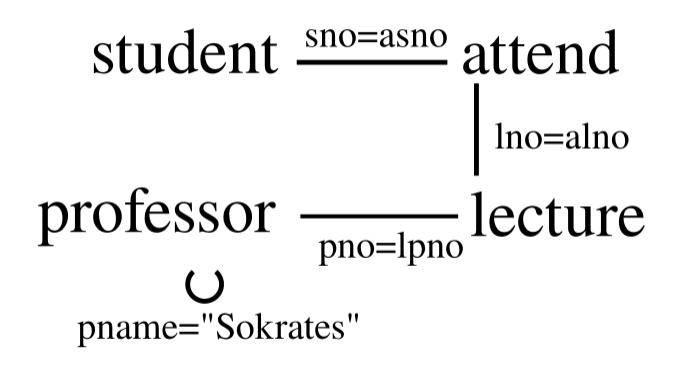
\includegraphics[width=.7\textwidth]{../images/db/2.png}
\label{}
\end{center}

\begin{center}
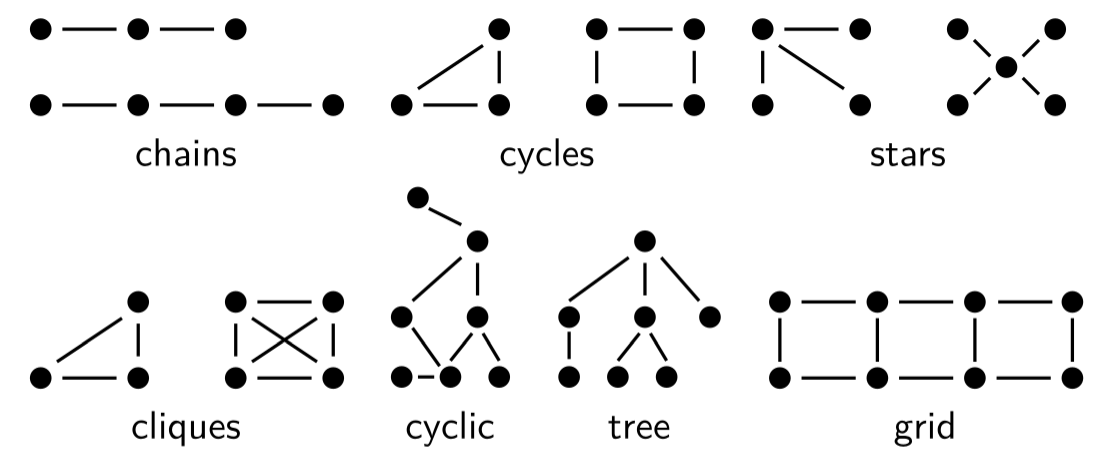
\includegraphics[width=.8\textwidth]{../images/db/3.png}
\captionof{figure}{\label{}Shapes of Query Graphs}
\end{center}



A join tree is a binary tree with
\begin{itemize}
\item join operators as inner nodes
\item relations as leaf nodes
\end{itemize}

Commonly used classes of join trees:
\begin{itemize}
\item left-deep tree
\item right-deep tree
\item zigzag tree
\item bushy tree
\end{itemize}
The first three are summariezed as \textbf{linear trees}

\textbf{Join selectivity}
\begin{itemize}
\item input
\begin{itemize}
\item cardinalities \(\abs{R_i}\)
\item selectivities \(f_{i,j}\): if \(p_{i,j}\) is the join predicate between \(R_i\) and \(R_j\), define
\begin{equation*}
f_{i,j}=\frac{R_i\bowtie_{p_{i,j}}R_j}{R_i\times R_j}
\end{equation*}
\end{itemize}
\item Calculate: \(\abs{R_i\bowtie_{p_{i,j}}R_j}=f_{i,j}\abs{R_i}\abs{R_j}\)
\item Rational: The selectivity can be computed/estimated easily (ideally)
\end{itemize}

Given a join tree \(T\), the result cardinality \(\abs{T}\) can be computed recursively as
\begin{equation*}
\abs{T}=
\begin{cases}
\abs{R_i}&\text{if $T$ is a leaf }R_i\\
(\displaystyle\prod_{R_i\in T_1,R_j\in T_2}f_{i,j})\abs{T_1}\abs{T_2}&\text{if }T=T_1\bowtie T_2
\end{cases}
\end{equation*}
assuming independence of the predicates

Given a join tree \(T\), the cost function \(C_{out}\) is defined as
\begin{equation*}
C_{out}(T)=
\begin{cases}
0&\text{if $T$ is a leaf }R_i\\
\abs{T}+C_{out}(T_1)+C_{out}(T_2)\text{if }T=T_1\bowtie T_2
\end{cases}
\end{equation*}

Consider nested loop join (nlj), hash join (hj), and sort merge join (smj), \cite{10.5555/645913.671481}
\begin{align*}
C_{nlj}(e_1\bowtie_pe_2)&\quad=\quad\abs{e_1}\abs{e_2}\\
C_{hj}(e_1\bowtie_pe_2)&\quad=\quad h\abs{e_1}\\
C_{smj}(e_1\bowtie_pe_2)&\quad=\quad\abs{e_1}\log(\abs{e_1})+\abs{e_2}\log(\abs{e_2})
\end{align*}
where \(e_i\) are join trees and \(h\) is the average length of the collision chain in the hash table. We
will assume \(h=1.2\).
\subsubsection{Search Space}
\label{sec:org218a7bf}
\subsubsection{Greedy Heuristics}
\label{sec:org1a4e861}
\subsubsection{IKKBZ}
\label{sec:orgd71b815}
\subsubsection{MVP}
\label{sec:orgd5f030a}
\subsubsection{Dynamic Programming}
\label{sec:orgc117908}
\subsubsection{Simplifying the Query Graph}
\label{sec:orge68e11b}
\subsubsection{Adaptive Optimization}
\label{sec:org5d16f82}
\subsubsection{Generating Permutations}
\label{sec:orge070c5a}
\subsubsection{Transformative Approaches}
\label{sec:orge148af1}
\subsubsection{Randomized Approaches}
\label{sec:org1fad68c}
\subsubsection{Metaheuristics}
\label{sec:org36893f1}
\subsubsection{Iterative Dynamic Programming}
\label{sec:orgd74f8f3}
\subsubsection{Order Preserving Joins}
\label{sec:orgc6f6829}
\subsubsection{Complexity of Join Processing}
\label{sec:orgcf294d8}
\subsection{Accessing the Data}
\label{sec:org264c3b4}

\subsection{Physical Properties}
\label{sec:orgb748054}

\subsection{Query Rewriting}
\label{sec:orgc40a8a3}

\subsection{Self Tuning}
\label{sec:orgfc8c880}
\section{Transaction System}
\label{sec:org45c2df0}
\subsection{Computational Models}
\label{sec:org55696af}
\subsubsection{Page Model}
\label{sec:org13e1f50}
\begin{definition}[Page Model Transaction]
A \textbf{transaction} \(t\) is a partial order of steps of the form \(r(x)\) or \(w(x)\)
where \(x\in D\) and reads and writes as well as multiple writes applied to the same object are
ordered. We write \(t=(op,<)\) for transaction \(t\) with step set \(op\) and partial order \(<\)
\end{definition}
\subsubsection{Object Model}
\label{sec:org2d241a2}
\begin{definition}[Object Model Transaction]
A \textbf{transaction} \(t\) is a (finite) tree of labeled nodes with
\begin{itemize}
\item the transaction identifier as the label of the root node,
\item the names and parameters of invoked operations as labels of inner nodes, and
\item page-model read/write operations as labels of leafs nodes, along with a partial order < on the
leaf nodes s.t. for all leaf-node operations \(p\) and \(q\) with \(p\) of the form \(w(x)\)
and \(q\) of the form \(r(x)\) or \(w(x)\) or vice versa, we have \(p<q\vee q<p\).
\end{itemize}
\end{definition}

\begin{center}
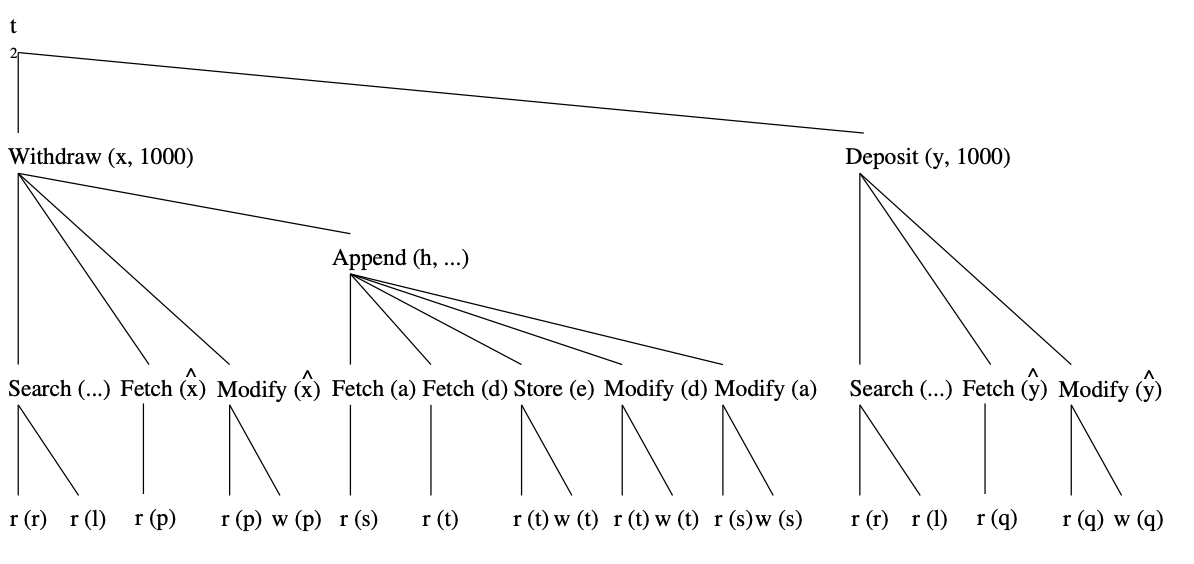
\includegraphics[width=.8\textwidth]{../images/bigdatabase/1.png}
\label{}
\end{center}
\subsection{Notions of Correctness for the Page Model}
\label{sec:org16ba78e}
\subsubsection{Canonical Synchronization Problems}
\label{sec:org9b83e85}

Lost Update Problem:
\begin{center}
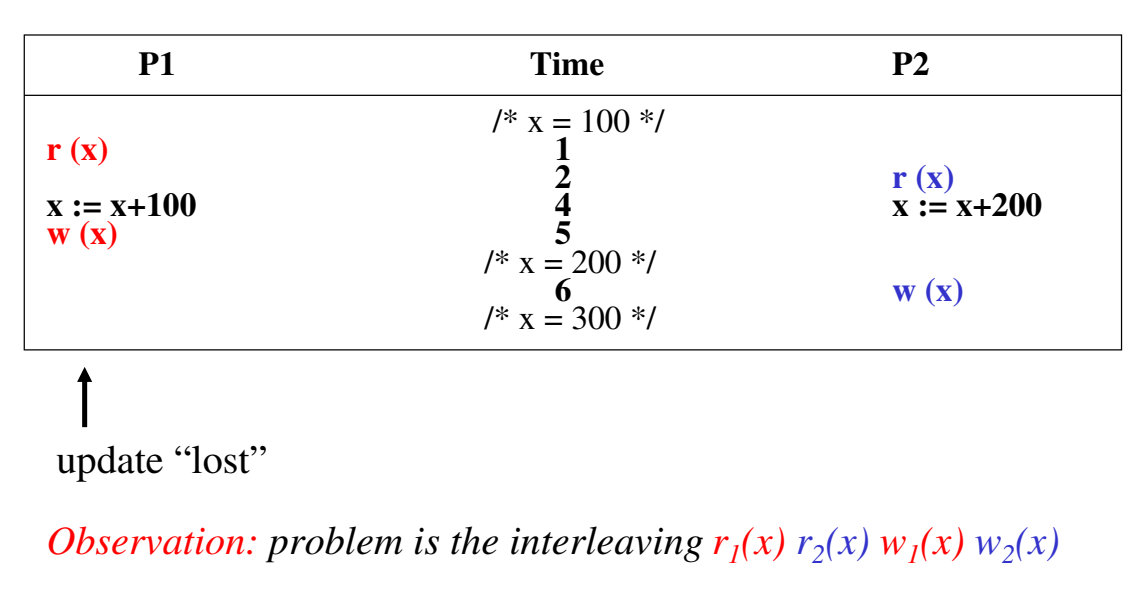
\includegraphics[width=.8\textwidth]{../images/bigdatabase/2.png}
\label{}
\end{center}

Inconsistent Read Problem
\begin{center}
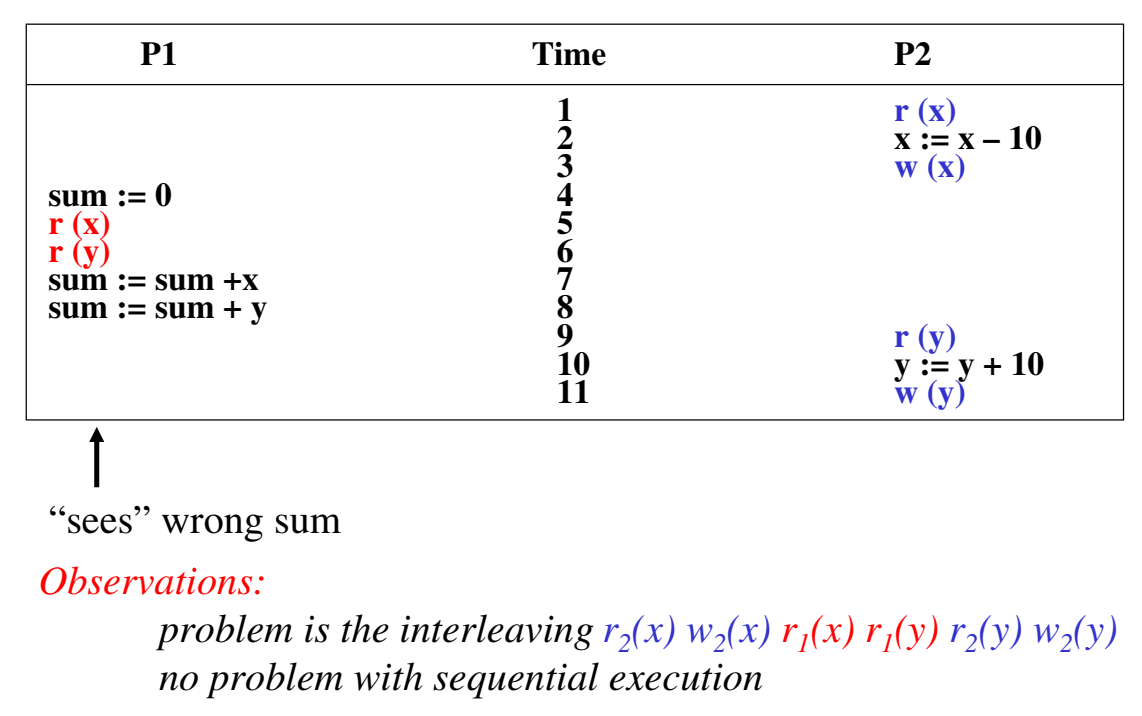
\includegraphics[width=.8\textwidth]{../images/bigdatabase/3.png}
\label{}
\end{center}

Dirty Read Problem
\begin{center}
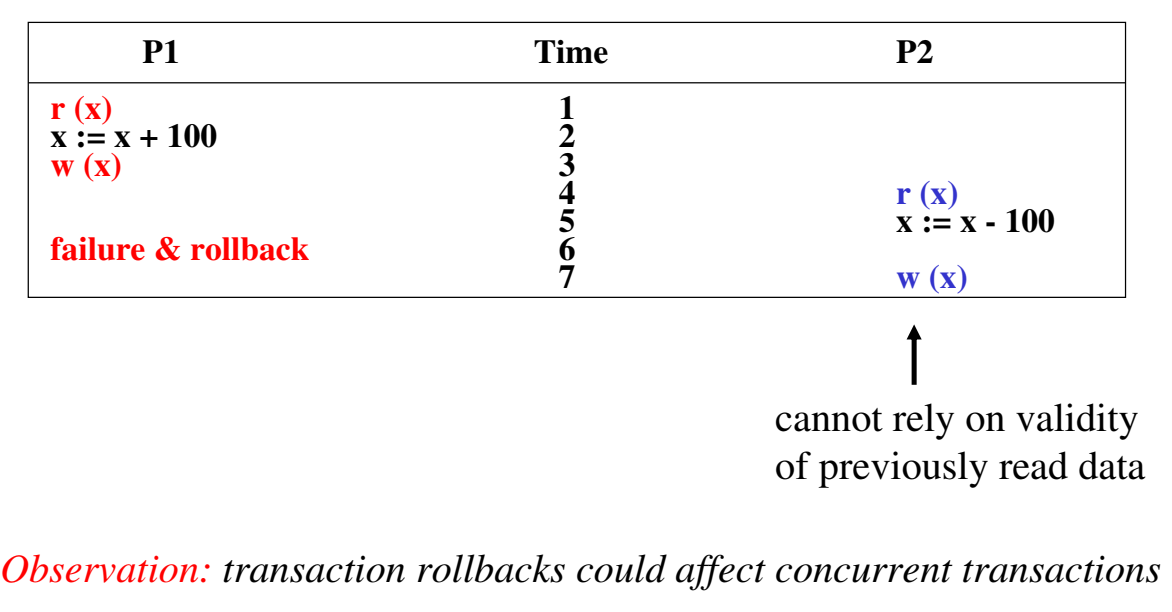
\includegraphics[width=.8\textwidth]{../images/bigdatabase/4.png}
\label{}
\end{center}
\subsubsection{Syntax of Histories and Schedules}
\label{sec:org6222a9e}
\begin{definition}[Schedules and histories]
Let \(T=\{t_1,\dots,t_n\}\) be a set of transactions, where each \(t_i\in T\) has the form
\(t_i=(op_i,<_i)\)
\begin{enumerate}
\item A \textbf{history} for \(T\) is a pair \(s=(op(s),<_s)\) s.t.
\begin{enumerate}
\item \(op(s)\subseteq\bigcup_{i=1}^nop_i\cup\bigcup_{i=1}^n\{a_i,c_i\}\)
\item for all \(1\le i\le n\), \(c_i\in op(s)\Leftrightarrow a_i\notin op(s)\)
\item \(\bigcup_{i=1}^n<_i\subseteq<_s\)
\item for all \(1\le i\le n\) and all \(p\in op_i\), \(p<_sc_i\vee p<_sa_i\)
\item for all \(p,q\in op(s)\) s.t. at least one of them is a write and both access the same
data item: \(p<_sq\vee q<_sp\)
\end{enumerate}
\item A \textbf{schedule} is a prefix of a history
\end{enumerate}
\end{definition}

\begin{definition}[]
A history \(s\) is \textbf{serial} if for any two transactions \(t_i\) and \(t_j\) in \(s\),
where \(i\neq j\), all operations from \(t_i\) are ordered in \(s\) before all operations
from \(t_j\) or vice versa
\end{definition}

\begin{definition}[]
\begin{itemize}
\item \(trans(s):=\{t_i\mid s\text{ contains step of }t_i\}\)
\item \(commit(s):=\{t_i\in trans(s)\mid c_i\in s\}\)
\item \(abort(s):=\{t_i\in trans(s)\mid a_i\in s\}\)
\item \(active(s):=trans(s)-(commit(s)\cup abort(s))\)
\end{itemize}
\end{definition}


\begin{center}
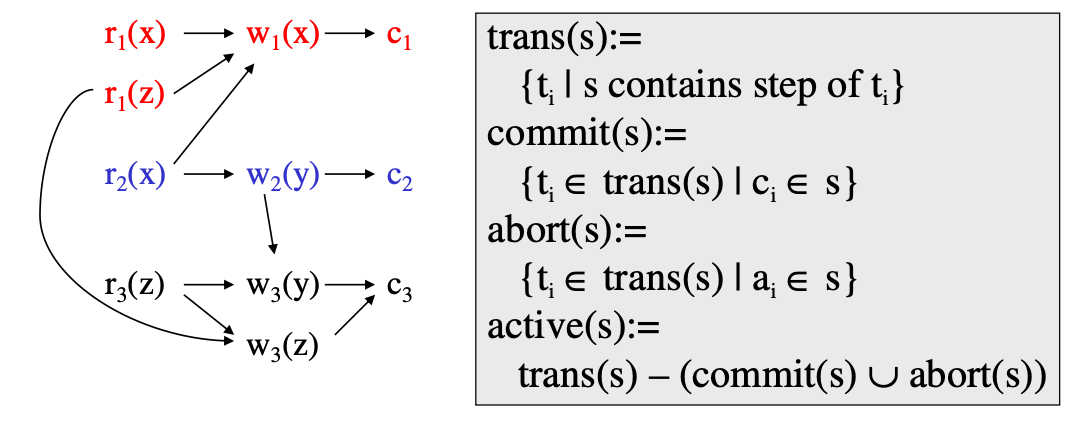
\includegraphics[width=.8\textwidth]{../images/bigdatabase/6.png}
\label{}
\end{center}

\begin{center}
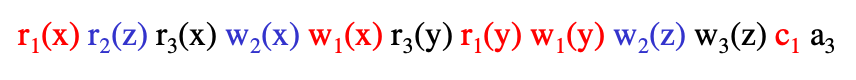
\includegraphics[width=.8\textwidth]{../images/bigdatabase/5.png}
\label{}
\end{center}
\subsubsection{Herbrand Semantics of Schedules}
\label{sec:org76b25ab}
\begin{definition}[Herbrand Semantics of Steps]
For schedule \(s\) the \textbf{Herbrand semantics} \(H_s\) of steps \(r_i(x),w_i(x)\in op(s)\) is :
\begin{enumerate}
\item \(H_s[r_i(x)]:=H_s[w_j(x)]\) where \(w_j(x)\) is the last write on \(x\) in \(s\)
before \(r_i(x)\)
\item \(H_s[w_i(x)]:=f_{ix}(H_x[r_i(y_1)],\dots,H_s[r_i(y_m)])\) where
the \(r_i(y_j)\), \(1\le j\le m\), are all read operations of \(t_i\) that occur in \(s\)
before \(w_i(x)\) and \(f_{ix}\) is an uninterpreted \(m\)-ary function symbol.
\end{enumerate}
\end{definition}

\begin{definition}[Herbrand Universe]
For data items \(D=\{x,y,z,\dots\}\) and transactions \(t_i\), \(1\le i\le n\), the \textbf{Herbrand
universe HU} is the smallest set of symbols s.t.
\begin{enumerate}
\item \(f_{0x}()\in HU\) for each \(x\in D\) where \(f_{0x}\) is a constant, and
\item if \(w_i(x)\in op_i\) for some \(t_i\), there are \(m\) read
operations \(r_i(y_1),\dots,r_i(y_m)\) that precede \(w_i(x)\) in \(t_i\),
and \(v_1,\dots,v_m\in HU\), then \(f_{ix}(v_1,\dots,v_m)\in HU\)
\end{enumerate}
\end{definition}

\begin{definition}[Schedule Semantics]
The \textbf{Herbrand semantics of a schedule} \(s\) is the mapping \(H[s]:D\to HU\) defined
by \(H[s](x):=H_s[w_i(x)]\) where \(w_i(x)\) is the last operation from \(s\) writing \(x\), for
each \(x\in D\)
\end{definition}

\begin{center}
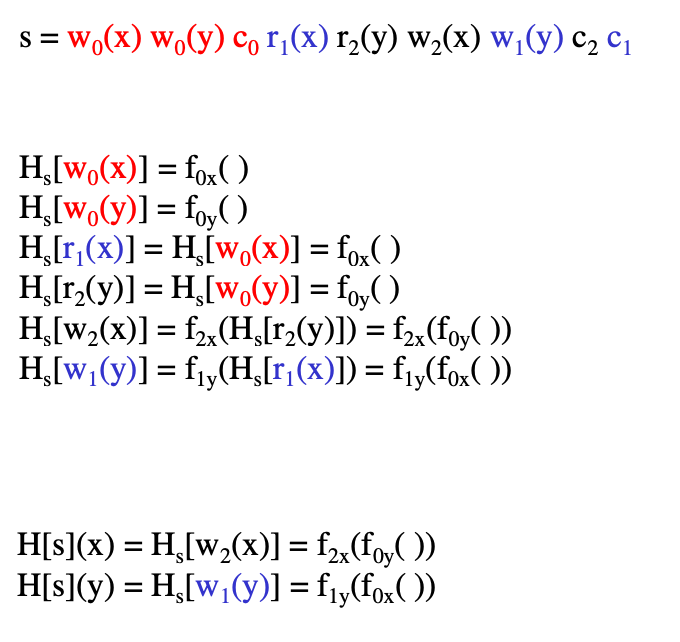
\includegraphics[width=.6\textwidth]{../images/bigdatabase/7.png}
\label{}
\end{center}
\subsubsection{Final-State Serializability}
\label{sec:org6d27359}
\begin{definition}[]
Schedules \(s\) and \(s'\) are called \textbf{final state equivalent}, denoted \(s\approx_fs'\)
if \(op(s)=op(s')\) and \(H[s]=H[s']\)
\end{definition}

\begin{center}
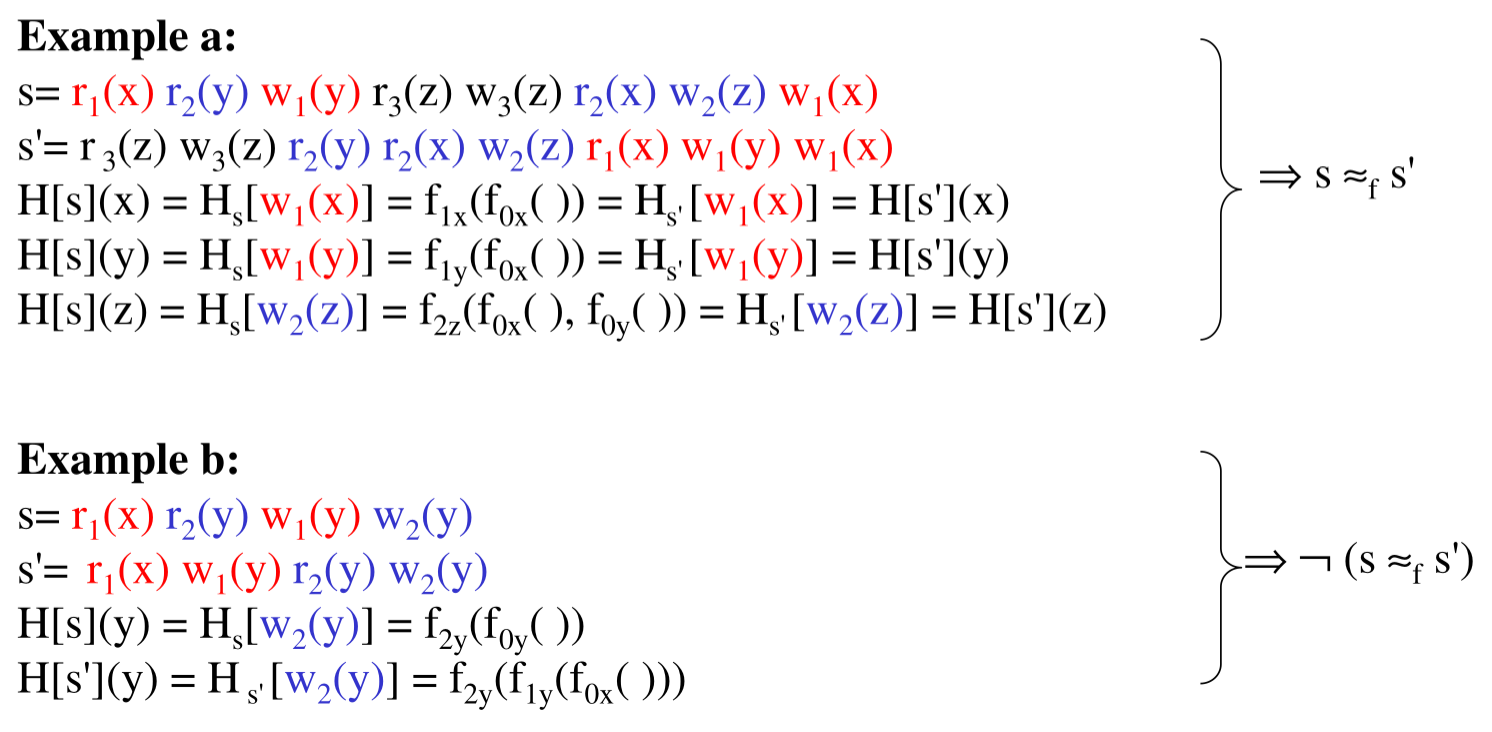
\includegraphics[width=.7\textwidth]{../images/bigdatabase/13.png}
\label{}
\end{center}

\begin{definition}[Reads-from Relation]
Given a schedule \(s\), extended with an initial and a final transaction, \(t_0\)
and \(t_\infty\)
\begin{enumerate}
\item \(r_j(x)\) \textbf{reads \(x\) in \(s\) from \(w_i(x)\)} if \(w_i(x)\) is the last write on \(x\)
s.t. \(w_i(x)<_sr_j(x)\)
\item The \textbf{reads-from relation} of \(x\) is
\begin{equation*}
RF(s):=\{(t_i,x,t_j)\mid \text{an }r_j(x)\text{ reads \(x\) from a }w_i(x)\}
\end{equation*}
\item Step \(p\) is \textbf{directly useful} for step \(q\), denoted \(p\to q\), if \(q\) reads from \(p\),
or \(p\) is a read step and \(q\) is a subsequent write step of the same
transaction. \(\to^*\), the \textbf{useful relation}, denotes the reflexive and transitive closure of \(\to\).
\item Step \(p\) is \textbf{alive} in \(s\) if it is useful for some step from \(t_\infty\), i.e.,
\begin{equation*}
(\exists q\in t_\infty)p\xrightarrow{*}q
\end{equation*}
and \textbf{dead} otherwise
\item The \textbf{live-reads-from relation} of \(s\) is
\begin{equation*}
LRF(s):=\{(t_i,x,t_j)\mid \text{an alive \(r_j(x)\) reads \(x\) from \(w_i(x)\)}\}
\end{equation*}
\end{enumerate}
\end{definition}

\begin{theorem}[]
For schedules \(s\) and \(s'\) the following statements hold:
\begin{enumerate}
\item \(s\approx_fs'\) iff \(op(s)=op(s')\) and \(LRF(s)=LRF(s')\)
\item For \(s\) let the step graph \(D(s)=(V,E)\) be a directed graph with vertices \(V:=op(s)\)
and edges \(E:=\{(p,q)\mid p\to q\}\), and the reduced step graph \(D_1(s)\) be derived
from \(D(s)\) by removing all vertices that correspond to dead steps. Then \(LRF(s)=LRF(s')\)
iff \(D_1(s)=D_1(s')\)
\end{enumerate}
\end{theorem}

\begin{proof}
For a given schedule \(s\), we can construct a ``step graph'' \(D(s)=(V,E)\) as follows
\begin{align*}
V&:=op(s)\\
E&:=\{(p,q)\mid p,q\in V,p\to q\}
\end{align*}
From a step graph \(D(s)\), a reduced step graph \(D_l(s)\) can be derived by dropping all vertices (and
thier incident edges) that represent dead steps. Then the following can be proven:
\begin{enumerate}
\item \(LRF(s)=LRF(s')\Leftrightarrow D_l(s)=D_l(s')\)

If \(D_l(s)\neq D_l(s')\), if there is \(r(x)\in D_l(s)\setminus D_l(s')\), then clearly \(LRF(s)\neq LRF(s')\); if
there is \(w_i(x)\in D_l(s)\setminus D_l(s')\), then \((t_i,x,t_\infty)\in LRF(s)\setminus LRF(s')\).

If \(LRF(s)\neq LRF(s')\), suppose \((t_i,x,t_j)\in LRF(s)\setminus LRF(s')\), then clearly \(D_l(s)\neq D_l(s')\)
\item \(s\approx_fs'\) iff \(op(s)=op(s')\) and \(D_l(s)=D_l(s')\)
\end{enumerate}
\end{proof}

\begin{corollary}[]
Final-state equivalence of two schedules \(s\) and \(s'\) can be decided in time that is
polynomial in the length of the two schedules.
\end{corollary}
\subsubsection{View Serializability}
\label{sec:org5bc1155}
As we have seen, FSR emphasizes steps that are alive in a schedule. However, since the semantics
of a schedule and of the transactions occurring in a schedule are unknown, it is reasonable to
require that in two equivalent schedules, each transaction reads the same values, independent of
its liveliness.

\textbf{Lost update anomaly}: \(L=r_1(x)r_2(x)w_1(x)w_2(x)c_1c_2\). History is not
FSR,
 \(LRF(L)=\{(t_0,x,t_2),(t_2,x,t_\infty)\}\),
 \(LRF(t_1t_2)=\{(t_0,x,t_1),(t_1,x,t_2),(t_2,x,t_\infty)\}\) and
 \(LRF(t_2t_1)=\{(t_0,x,t_2),(t_2,x,t_1),(t_1,x,t_\infty)\}\)


\textbf{Inconsistent read anomaly}: \(I=r_2(x)w_2(x)r_1(x)r_1(y)r_2(y)w_2(y)c_1c_2\), history is FSR
\(LFR(I)=LFR(t_1t_2)=LFR(t_2t_1)=\{(t_0,x,t_2),(t_0,y,t_2),(t_2,x,t_\infty),(t_2,y,t_\infty)\}\)


\begin{definition}[View Equivalence]
Schedules \(s\) and \(s'\) are \textbf{view equivalent}, denoted \(s\approx_vs'\), if the following
hold:
\begin{enumerate}
\item \(op(s)=op(s')\)
\item \(H[s]=H[s']\)
\item \(H_s[p]=H_{s'}[p]\) for all (read or write) steps
\end{enumerate}
\end{definition}

\begin{theorem}[]
For schedules \(s\) and \(s'\) the following statements hold.
\begin{enumerate}
\item \(s\approx_v s'\) iff \(op(s)=op(s')\) and \(RF(s)=RF(s')\)
\item \(s\approx_vs'\) iff \(D(s)=D(s')\)
\end{enumerate}
\end{theorem}

\begin{proof}
\begin{enumerate}
\item \(\Rightarrow\): Consider a read step \(r_i(x)\) from \(s\).
Then \(H_s[r_i(x)]=H_{s'}[r_i(x)]\) implies that if \(r_i(x)\) reads from some
step \(w_j(x)\) in \(s\), the same holds in \(s'\), and vice versa.

\(\Leftarrow\): If \(RF(s)=RF(s')\), this in particular applies to \(t_\infty\);
hence \(H[s]=H[s']\). Similarly, for all other reads \(r_i(x)\) in \(s\), we
have \(H_s[r_i(x)]=H_{s'}[r_i(x)]\).

Suppose for some \(w_i(x)\), \(H_s[w_i(x)]\neq H_{s'}[w_i(x)]\). Thus the set of values read
by \(t_i\) prior to step \(w_i\) is different in \(s\) and \(s'\), a contradiction to our
assumption that \(RF(s)=RF(s')\).
\end{enumerate}
\end{proof}

\begin{corollary}[]
View equivalence of two schedules \(s\) and \(s'\) can be decided in time that is polynomial in
the length of the two schedules
\end{corollary}

\begin{definition}[]
A schedule \(s\) is \textbf{view serializable} if there exists a serial schedule \(s'\)
s.t. \(s\approx_vs'\). VSR denotes the class of all view-serializable histories
\end{definition}

\begin{theorem}[]
\(VSR\subset FSR\)
\end{theorem}

\begin{theorem}[]
Let \(s\) be a history without dead steps. Then \(s\in VSR\) iff \(s\in FSR\)
\end{theorem}

\begin{theorem}[]
The problem of deciding for a given schedule \(s\) whether \(s\in VSR\) holds is NP-complete
\end{theorem}

\begin{definition}[Monotone Classes of Histories]
Let \(s\) be a schedule and \(T\subseteq trans(s)\). \(\pi_T(s)\) denotes the projection
of \(s\) onto \(T\). A class of histories is called \textbf{monotone} if the following holds:
\begin{center}
If \(s\) is in \(E\), then \(\Pi_T(s)\) is in \(E\) for each \(T\subseteq trans(s)\)
\end{center}
\end{definition}

VSR is not monotone
\subsubsection{Conflict Serializability}
\label{sec:orgb94d917}
\begin{definition}[Conflicts and Conflict Relations]
Let \(s\) be a schedule, \(t,t'\in trans(s)\), \(t\neq t'\)
\begin{enumerate}
\item Two data operations \(p\in t\) and \(q\in t'\) are in \textbf{conflict} in \(s\) if
they access the same data item and at least one of them is a write
\item \(conf(s):=\{(p,q)\mid p,q\text{ are in conflict and }p<_sq\}\) is the \textbf{conflict relation} of \(s\)
\end{enumerate}
\end{definition}

\begin{definition}[]
Schedules \(s\) and \(s'\) are \textbf{conflict equivalent}, denoted \(s\approx_cs'\),
if \(op(s)=op(s')\) and \(conf(s)=conf(s')\)
\end{definition}

\begin{definition}[]
Schedule \(s\) is \textbf{conflict serializable} if there is a serial schedule \(s'\)
s.t. \(s\approx_cs'\). CSR denotes the class of all conflict serializable schedules.
\end{definition}

\begin{theorem}[]
\(CSR\subset VSR\)
\end{theorem}

\index{conflict graph}
\begin{definition}[]
Let \(s\) be a schedule. The \textbf{conflict graph} \(G(s)=(V,E)\)  is a directed graph with
vertices \(V:=commit(s)\) and
edges \(E:=\{(t,t')\mid t\neq t'\text\wedge\exists p\in t,q\in t':(p,q)\in conf(s)\}\)
\end{definition}

\begin{theorem}[]
Let \(s\) be a schedule. Then \(s\in CSR\) iff \(G(s)\) is acyclic.
\end{theorem}

\begin{proof}
\(\Rightarrow\): There is a serial history \(s'\) s.t. \(op(s)=op(s')\)
and \(conf(s)=conf(s')\). Consider \(t,t'\in V\), \(t\neq t'\) with \((t,t')\in E\). Then we
have
\begin{equation*}
(\exists p\in t)(\exists q\in t')p<_sq\wedge(p,q)\in conf(s)
\end{equation*}
Then \(p<_{s'}q\). Also all of \(t\) occur before all of \(t'\) in \(s'\).

Suppose \(G(s)\) were cyclic. Then we have a cycle \(t_1\to t_2\to\dots\to t_k\to t_1\). The
same cycle also exists in \(G(s')\), a contradiction

\(\Leftarrow\):
\end{proof}

\begin{corollary}[]
Testing if a schedule is in CSR can be done in time polynomial to the schedule's number of transactions
\end{corollary}

Commutativity rules:
\begin{enumerate}
\item \(C_1:r_i(x)r_j(y)\sim r_j(y)r_i(x)\) if \(i\neq j\)
\item \(C_2:r_1(x)w_j(y)\sim w_j(y)r_i(x)\) if \(i\neq j\) and \(x\neq y\)
\item \(C_3:w_i(x)w_j(y)\sim w_j(y)w_i(x)\) if \(i\neq j\) and \(x\neq y\)
\end{enumerate}
Ordering rule:
\begin{enumerate}
\setcounter{enumi}{3}
\item \(C_4\): \(o_i(x)\), \(p_j(y)\) unordered \(\Rightarrow\) \(o_i(x)p_j(y)\)
if \(x\neq y\) or both \(o\) and \(p\) are reads
\end{enumerate}


\begin{definition}[]
Schedules \(s\) and \(s'\) s.t. \(op(s)=op(s')\) are \textbf{commutativity based equivalent},
denoted \(s\sim^*s'\), if \(s\) can be transformed into \(s'\) by applying rules C1, C2, C3, C4 finitely.
\end{definition}

\begin{theorem}[]
Let \(s\) and \(s'\)  be schedules s.t. \(op(s)=op(s')\). Then \(s\approx_cs'\) iff \(s\sim^*s'\)
\end{theorem}

\begin{definition}[]
Schedule \(s\) is \textbf{commutativity-based reducible} if there is a serial schedule \(s'\) s.t. \(s\sim^*s'\)
\end{definition}

\begin{corollary}[]
Schedule \(s\) is commutativity-based reducible iff \(s\in CSR\)
\end{corollary}

\begin{definition}[]
Schedule \(s\) is \textbf{order preserving conflict serializable} if it is conflict equivalent to a
serial schedule \(s'\) and for all \(t,t'\in trans(s)\), if \(t\) completely precedes \(t'\)
in \(s\), then the same holds in \(s'\). OSCR denotes the class of all schedules with this property.
\end{definition}

\begin{theorem}[]
\(OCSR\subset CSR\)
\end{theorem}

\(s=w_1(x)r_2(x)c_2w_c(y)c_3w_1(y)c_1\in CSR\setminus OCSR\)


\begin{definition}[]
Schedules \(s\) is \textbf{commit order preserving conflict serializable} if for
all \(t_i,t_j\in trans(s)\), if there are \(p\in t_i\), \(q\in t_j\) with \((p,q)\in conf(s)\),
then \(c_i<_sc_j\).

COCSR denotes the class of all schedules with this property
\end{definition}

\begin{theorem}[]
\(COCSR\subset CSR\)
\end{theorem}

\begin{theorem}[]
Schedule \(s\) is in COCSR iff there is a serial schedule \(s'\) s.t. \(s\approx_cs'\) and for
all \(t_i,t_j\in trans(s)\): \(t_i<_{s'}t_j\Leftarrow c_i<_{s}c_j\)
\end{theorem}
\subsubsection{Commit Serializability}
\label{sec:org530c33d}
\subsubsection{An Alternative Criterion: Interleaving Specifications}
\label{sec:orgb0f6bc3}
\subsection{Concurrency Control Algorithms}
\label{sec:org558a237}
\subsubsection{General Scheduler Design}
\label{sec:org075ac35}
\begin{center}
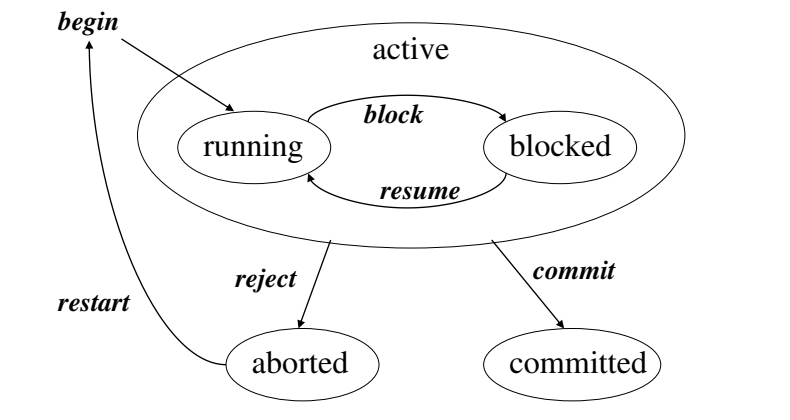
\includegraphics[width=.8\textwidth]{../images/bigdatabase/8.png}
\label{}
\end{center}

\begin{definition}[CSR Safety]
For a scheduler \(S\), \(Gen(S)\) denotes the set of all schedules that \(S\) can generate. A
scheduler is called \textbf{CSR safe} if \(Gen(S)\subseteq CSR\)
\end{definition}

\begin{center}
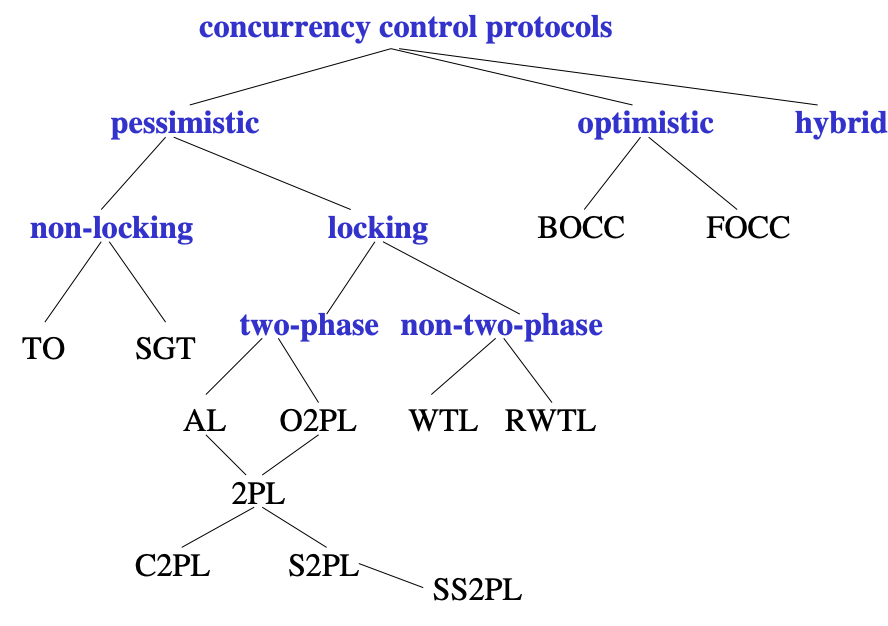
\includegraphics[width=.8\textwidth]{../images/bigdatabase/9.png}
\label{}
\end{center}
\subsubsection{Locking Schedulers}
\label{sec:org4425226}
\begin{enumerate}
\item Introduction
\label{sec:orgb47d1f9}
General locking rules:
\begin{enumerate}
\item Each data operation \(o_i(x)\) must be preceded by \(ol_i(x)\) and followed by \(ou_i(x)\)
\item For each \(x\) and \(t_i\) there is at most one \(ol_i(x)\) and at most one \(ou_i(x)\)
\item No \(ol_i(x)\)  or \(ou_i(x)\) is redundant
\item If \(x\) is locked by both \(t_i\) and \(t_j\), then these locks are compatible
\end{enumerate}

Let \(\DT(s)\) denote the projection of \(s\) onto the steps of type \(r,w,a,c\). \(\CP(s)\)
denotes the committed projection of \(s\).
\item Two-Phase Locking
\label{sec:org21d52c9}
\begin{definition}[]
A locking protocol is \textbf{two-phase} if for every output schedule \(s\) and every
transaction \(t_i\in trans(s)\) no \(ql_i\) step follows the first \(ou_i\) step (\(q,0\in\{r,w\}\))
\end{definition}
\begin{center}
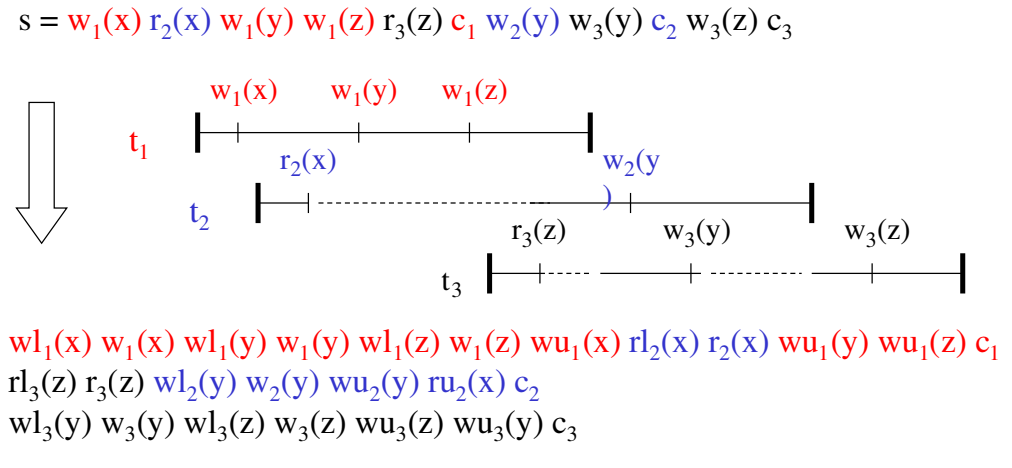
\includegraphics[width=.8\textwidth]{../images/bigdatabase/10.png}
\label{}
\end{center}


\begin{lemma}[]
\label{4.1}
Let \(s\) be the output of a 2PL scheduler. Then for each transaction \(t_i\in commit(DT(s))\), the
following holds:
\begin{enumerate}
\item if \(o_i(x)\), \(o\in\{r,w\}\), occurs in \(\CP(\DT(s))\), then so do \(ol_i(x)\) and \(ou_i(x)\)
with the sequencing \(ol_i(x)<o_i(x)<ou_i(x)\).
\item If \(t_j\in\commit(\DT(s))\), \(i\neq j\), is another transaction s.t. some steps \(p_i(x)\)
and \(q_j(x)\) from \(\CP(\DT(s))\) are in conflict, then either \(pu_i(x)<ql_j\)
or \(qu_j(x)<pl_i(x)\) holds.
\item If \(p_i(x)\) and \(q_j(y)\) are in \(\CP(\DT(s))\), then \(pl_i(x)<qu_i(y)\), i.e., every lock
operation occurs before every unlock operation of the same transaction.
\end{enumerate}
\end{lemma}

\begin{lemma}[]
\label{4.2}
Let \(s\) be the output of a 2PL scheduler, and let \(G:=G(\CP(\DT(s)))\) be the conflict graph
of \(\CP(\DT(s))\), then the following holds:
\begin{enumerate}
\item If \((t_i,t_j)\) is an edge in \(G\), then \(pu_i(x)<ql_j(x)\) for some data item \(x\) and two
operations \(p_i(x)\), \(q_j(x)\) in conflict.
\item If \((t_1,\dots,t_n)\) is a path in \(G\), \(n\ge 1\), then \(pu_1(x)<ql_n(y)\) for two data
items \(x\) and \(y\) as well as operations \(p_1(x)\) and \(q_n(y)\).
\item \(G\) is acyclic.
\end{enumerate}
\end{lemma}

Since the conflict graph of an output produced by a 2PL scheduler is acyclic, we have

\begin{theorem}[]
\(Gen(2PL)\subset CSR\)
\end{theorem}

\begin{examplle}[Strict inclusion]
Let \(s=w_1(x)r_2(x)c_2r_3(y)c_3w_1(y)c_1\). \(s\in\CSR\) as \(s\approx_ct_3t_1t_2\). And \(s\) cannot be produced
by a 2PL scheduler
\end{examplle}

\begin{theorem}[]
\(Gen(2PL)\subset OCSR\)
\end{theorem}
\item Deadlock Handling
\label{sec:org17e1cfd}
Deadlock detection:
\begin{enumerate}
\item maintain dynamic \textbf{waits-for graph} (WFG) with active transactions as nodes and an edge
from \(t_i\) to \(t_j\) if \(t_j\) waits for a lock held by \(t_i\)
\item Test WFG for cycles
\end{enumerate}

Deadlock resolution: Choose a transaction on a WFG cycles as a \textbf{deadlock victim} and abort this
transaction, and repeat until no more cycles.

Possible victim selection strategies:
\begin{enumerate}
\item Last blocked
\item Random
\item Youngest
\item Minimum locks
\item Minimum work
\item Most cycles
\item Most edges
\end{enumerate}

Deadlock Prevention: Restrict lock waits to ensure acyclic WFG at all times. Reasonable deadlock
prevention strategies when \(t_i\) is blocked by \(t_j\):
\begin{enumerate}
\item \textbf{wait-die}: if \(t_i\) started before \(t_j\) then wait else abort \(t_i\).
\item \textbf{wound-wait}: if \(t_i\) started before \(t_j\) then abort \(t_i\) else wait
\item \textbf{Immediate restart}: abort \(t_i\)
\item \textbf{Running priority}: if \(t_j\) is itself blocked then abort \(t_j\) else wait
\item \textbf{Timeout}: abort waiting transaction when a timer expires.
\end{enumerate}
Abort entails later restart
\item Variants of 2PL
\label{sec:org90f2dd7}
\begin{definition}[]
Under \textbf{static} or \textbf{conservative 2PL} (C2PL) each transaction acquires all its locks before the first
data operation.
\end{definition}

\begin{center}
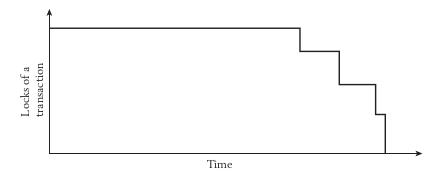
\includegraphics[width=.7\textwidth]{../images/bigdatabase/11.png}
\captionof{figure}{\label{}Conservative 2PL}
\end{center}

\begin{definition}[]
Under \textbf{strict 2PL} (S2PL) each transaction holds all its write locks until the transaction terminates.
\end{definition}

\begin{center}
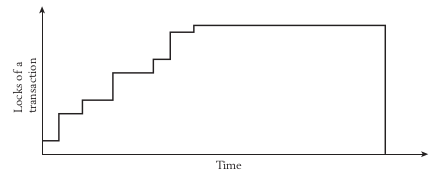
\includegraphics[width=.7\textwidth]{../images/bigdatabase/12.png}
\captionof{figure}{\label{}Strict 2PL}
\end{center}

\begin{definition}[]
Under \textbf{strong 2PL} (SS2PL) each transaction holds all its locks until the transaction terminates
\end{definition}

\begin{theorem}[]
\(\Gen(SS2PL)\subset\Gen(S2PL)\subset\Gen(2PL)\)
\end{theorem}

\begin{theorem}[]
\(\Gen(SS2PL)\subset COCSR\)
\end{theorem}
\item Ordered Sharing of Locks (O2PL)
\label{sec:org8faf339}
\item Altruistic Locking (AL)
\label{sec:org0def3fc}
\item Non-Two-Phase Locking (WTL, RWTL)
\label{sec:org48193b7}
Motivation: concurrent executions of transactions with access patterns that comply with
organizing data items into a virtual tree
\begin{align*}
&t_1=w_1(a)w_1(b)w_1(d)w_1(e)w_1(i)w_1(k)\\
&t_2=w_2(a)w_2(b)w_2(c)w_2(d)w_2(h)
\end{align*}
\begin{center} \begin{forest}
[a
    [b
        [c
            [f] [g]]
        [d [h]]
        [e
            [i
                [j] [k]]]]]
\end{forest}\end{center}

\begin{definition}[Write-only Tree Locking (WTL)]
Lock requests and releases must obey LR1 - LR4 and the following additional rules
\begin{enumerate}
\item WTL1: A lock on a node \(x\) other than the tree root can be acquired only if the transaction
already holds a lock on the parent of \(x\)
\item WTL2: After a \(wu_i(x)\) no further \(wl_i(x)\) is allowed
\end{enumerate}
\end{definition}
\item Geometry of Locking
\label{sec:orgc8546bd}
\end{enumerate}
\subsubsection{Non-Locking Schedulers}
\label{sec:orgcc3055f}
\begin{enumerate}
\item Timestamp Ordering
\label{sec:org7897099}
\end{enumerate}
\subsubsection{Hybrid Protocols}
\label{sec:org93d9c07}
\subsection{Multiversion Concurrency Control}
\label{sec:org86fa38d}
\subsubsection{Multiversion Schedules}
\label{sec:org983cc25}
\begin{examplle}[]
\(s=r_1(x)w_1(x)r_2(x)w_2(y)r_1(y)w_1(z)c_1c_2\notin\CSR\)
\end{examplle}
but schedule would be tolerable if \(r_1(y)\) could read the old version \(y_0\) of \(y\) to be
consistent with \(r_1(x)\)

Approach:
\begin{itemize}
\item each \(w\) step creates a new version
\item each \(r\) step can choose which version it wants/needs to read
\item versions are transparent to application and transient
\end{itemize}


\begin{definition}[]
Let \(s\) be a history with initial transaction \(t_0\) and final transaction \(t_\infty\). A
\textbf{version function} for \(s\) is a function \(h\) which associates with each read step of \(s\) a
previous write step on the same data item, and the identity for writes.
\end{definition}

\begin{definition}[]
A \textbf{multiversion (mv) history} for transactions \(T=\{t_1,\dots,t_n\}\) is a pair \(m=(\op(m),<_m)\)
where \(<_m\) is an order on \(\op(m)\) and
\begin{enumerate}
\item \(\op(m)=\bigcup_{i=1,\dots,n}h(\op(t_i))\) for some version function \(h\)
\item for all \(t\in T\) and all \(p,q\in\op(t_i)\): \(p<_tq\Rightarrow h(p)<_mh(q)\)
\item if \(h(r_j(x))=w_j(x_i)\), \(i\neq j\), then \(c_i\) is in \(m\) and \(c_i<_mc_j\)
\end{enumerate}
A \textbf{multiversion (mv) schedule} is a prefix of a multiversion history
\end{definition}

\begin{definition}[]
A multiversion schedule is a \textbf{monoversion schedule} if its version function maps each read to the
last preceding write on the same data item.
\end{definition}
\subsubsection{Multiversion Serializability}
\label{sec:org897cdb5}
\begin{definition}[]
For mv schedule \(m\) the reads-from relation of \(m\) is \(\RF(m)=\{(t_i,x,t_j)\mid r_j(x_i)\in\op(m)\}\)
\end{definition}

\begin{definition}[]
mv histories \(m\) and \(m'\) with \(trans(m)=trans(m')\) are \textbf{view equivalent}, \(m\equiv_vm'\), if \(\RF(m)=\RF(m')\)
\end{definition}
\subsubsection{Limiting the Number of Versions}
\label{sec:orgbd88af2}
\subsubsection{Multiversion Concurrency Control Protocols}
\label{sec:org713af3b}
\end{document}
